\documentclass[letterpaper,10pt,conference]{ieeeconf}
\IEEEoverridecommandlockouts
\overrideIEEEmargins

\usepackage{cite}
\usepackage{amsmath,amssymb,amsfonts}
\usepackage{algorithmic}
\usepackage{graphicx}
\usepackage{textcomp}
\usepackage{xcolor}

% additional packages
\usepackage{balance}
\usepackage{booktabs}
\usepackage{mathtools,mathrsfs,optidef}
\mathtoolsset{showonlyrefs=true}

\newtheorem{definition}{Definition}
\newtheorem{assumption}{Assumption}
\newtheorem{theorem}{Theorem}
\newtheorem{proposition}{Proposition}
\newtheorem{lemma}{Lemma}
\newtheorem{corollary}{Corollary}
\newtheorem{remark}{Remark}

\newcommand{\C}{\mathbb{C}}
\newcommand{\R}{\mathbb{R}}
\newcommand{\Z}{\mathbb{Z}}
\newcommand{\N}{\mathbb{N}}
\DeclareMathOperator{\argmax}{arg\,max}
\DeclareMathOperator{\argmin}{arg\,min}
\DeclareMathOperator{\diag}{diag}
\DeclareMathOperator{\rank}{rank}
\DeclareMathOperator{\tr}{tr}

\usepackage{tikz}
\usetikzlibrary{arrows.meta,calc,positioning,shapes}
\tikzset{
  every node/.style = {outer sep=0.12cm, inner sep=0},
  arrow/.style = {-{Triangle[length=0.25cm]}, thick},
  line/.style = {thick},
  block/.style = {rectangle, draw, minimum height=0.8cm, minimum width=2cm, thick, outer sep=0},
  sum/.style = {thick, circle, draw, inner sep=0, minimum size=6pt, outer sep=0},
  point/.style = {radius=2pt}
}

\newcommand{\T}{\top}
\newcommand{\graph}{\mathcal{G}}

\title{\LARGE\textbf{Distributed Event-Triggered Consensus Control of Discrete-Time Linear Multi-Agent Systems under LQ Performance Constraints}}

\author{Shumpei~Nishida and Kunihisa~Okano%
  \thanks{This work was supported by JST SPRING Grant Number JPMJSP2101 and JSPS KAKENHI Grant Number 25K01453.}
  \thanks{The authors are with the Graduate School of Science and Engineering,
    Ritsumeikan University,
    Shiga 525-8577 Japan.
    E-mails: {\footnotesize \{\texttt{re0158ff@ed.}, \texttt{kokano@fc.}\}%
    \texttt{ritsumei.ac.jp}}.}
}

\begin{document}

\maketitle
\thispagestyle{empty}
\pagestyle{empty}

\begin{abstract}
% This paper proposes a distributed event-triggered control method that not only guarantees consensus of multi-agent systems but also satisfies a prescribed LQ performance constraint.
% Taking the standard distributed control scheme with all-time communication as a baseline, we consider the problem of designing an event-triggered communication rule such that the resulting LQ cost satisfies a performance constraint with respect to the baseline cost while consensus is achieved.
% For general linear agents over an undirected graph, we employ local state predictors and a local triggering condition based only on information available to each agent.
% We then derive a sufficient condition for the proposed method to satisfy the performance constraint and guarantee consensus.
% In addition, we develop a tractable parameter design method for selecting the triggering parameters offline.
% Numerical examples demonstrate the effectiveness of the proposed method.
This paper proposes a distributed event-triggered control method that not only guarantees consensus of multi-agent systems but also satisfies a given LQ performance constraint.
Taking the standard distributed control scheme with all-time communication as a baseline, we consider the problem of designing an event-triggered communication rule such that the resulting LQ cost satisfies a performance constraint with respect to the baseline cost while consensus is achieved.
The main difficulty is that the performance requirement is global, whereas triggering decisions are made locally and asynchronously by individual agents, which cannot directly evaluate the global performance degradation.
To address this issue, we decompose allowable degradation across agents and design a triggering rule that uses only locally available information to satisfy the given LQ performance constraint.
For general linear agents on an undirected graph, we derive a sufficient condition that guarantees both consensus and the prescribed performance level.
We also develop a tractable offline design method for the triggering parameters.
Numerical examples illustrate the effectiveness of the proposed method.
\end{abstract}

\section{Introduction}

% Distributed and cooperative control of multi-agent systems has been extensively studied over the last decades because of its broad applications, such as vehicle formation \cite{ren2008distributed} and power networks \cite{bidram2014distributed}.
% In particular, the consensus problem, which aims to make all agents reach agreement through local information exchange \cite{olfati2007consensus}, is one of the fundamental problems in cooperative control and continues to attract significant attention \cite{hengster2013synchronization,jiao2019suboptimality,feng2021consensusability,yuan2025resilient}.
% However, when communication among agents is implemented over digital networks, frequent information exchange is often impractical due to limited communication resources.
% This has motivated the development of distributed event-triggered control for multi-agent systems, in which information transmissions among agents are executed only when certain conditions are satisfied, thereby reducing unnecessary communication while achieving the control objective \cite{garcia2014decentralized,nowzari2019event,mishra2023event}.
% With appropriately designed triggering rules, this approach can guarantee consensus with intermittent information exchange and significantly reduce the number of transmissions compared with all-time communication schemes.

% Despite these advances, many existing studies on distributed event-triggered control primarily focus on consensus, leaving limited analysis of the control performance achieved under event-triggered communication.
% Since consensus only describes whether the agents asymptotically reach agreement, it does not directly quantify closed-loop performance, such as transient response.
% To address this issue, several studies have explicitly examined the control performance of distributed event-triggered consensus using quadratic performance criteria \cite{meister2022analysis,meister2024time,antunes2023consistent,meister2026improving}.
% In \cite{meister2022analysis} and \cite{meister2024time}, time-triggered and event-triggered consensus control methods are compared under equal average communication rates using performance measures that quantify deviation from consensus.
% These studies show that, in the specific situation, time-triggered control can outperform event-triggered control when the number of agents is sufficiently large.
% In contrast, \cite{antunes2023consistent} considers a consensus problem for discrete-time integrators on a complete graph with a disagreement-based cost, and proposes an event-triggered strategy that achieves a lower cost than the time-triggered one under the same average communication rate.
% Building on \cite{meister2024time} and \cite{antunes2023consistent}, \cite{meister2026improving} shows that using more local information at the controllers improves closed-loop performance, but can eliminate the performance advantage of event-triggered control over time-triggered control.
% While these studies clarify certain performance properties of distributed event-triggered consensus control, their analyses are limited to simplified settings, such as single-integrator dynamics, special communication graphs, and performance criteria that only quantify disagreement among agents.

Distributed and cooperative control of multi-agent systems has been studied extensively because of its broad applications, including vehicle formation \cite{ren2008distributed} and power networks \cite{bidram2014distributed}.
In particular, the consensus problem, which aims to make all agents reach agreement through local information exchange \cite{olfati2007consensus}, is one of the fundamental problems and continues to attract significant attention \cite{hengster2013synchronization,jiao2019suboptimality,feng2021consensusability,yuan2025resilient}.
However, when communication among agents is implemented over digital networks, frequent information exchange is often impractical due to limited communication resources.
This motivates distributed event-triggered control, in which agents transmit information only when prescribed conditions are satisfied, thereby reducing unnecessary communication while achieving consensus \cite{garcia2014decentralized,hu2015consensus,nowzari2019event,mishra2023event}.

Despite this progress, most existing studies on distributed event-triggered consensus control focus mainly on whether consensus is achieved, with only limited analysis of control performance under event-triggered communication.
Since consensus only describes whether the agents asymptotically reach agreement, it does not directly quantify closed-loop performance, such as transient behavior.
To address this limitation, several studies have examined the control performance of distributed event-triggered consensus control using quadratic performance criteria \cite{meister2022analysis,meister2024time,antunes2023consistent,meister2026improving}.
For example, \cite{meister2022analysis} and \cite{meister2024time} show that time-triggered control can outperform event-triggered control in some settings, whereas \cite{antunes2023consistent} proposes an event-triggered control method that achieves a lower cost than time-triggered control.
Moreover, \cite{meister2026improving} shows that using more local information can improve closed-loop performance but eliminate the performance advantage of event-triggered control.
Although these studies clarify performance properties of event-triggered consensus control, they are limited to simplified settings, such as integrator dynamics, special communication graphs, and performance criteria that quantify only disagreement among agents.
Therefore, it remains unclear how to design distributed event-triggered communication mechanisms for general linear multi-agent systems with explicit performance guarantees.

% % This paper addresses distributed event-triggered consensus from a synthesis viewpoint rather than a performance analysis viewpoint.
% In this paper, we develop a distributed event-triggered consensus control method for general linear multi-agent systems that guarantees a prescribed level of LQ performance.
% We employ a quadratic performance criterion that quantifies both disagreement among agents and input energy, and formulate the consensus problem under an LQ performance constraint with respect to a baseline distributed control scheme with all-time communication.
% Unlike existing studies \cite{meister2022analysis,meister2024time,antunes2023consistent,meister2026improving}, our approach is not restricted to integrator dynamics or performance criteria that measure only disagreement.
% More importantly, the proposed triggering rule is derived explicitly from LQ performance degradation, rather than from a conventional norm-based threshold designed solely for consensus.
% As pointed out in \cite{garcia2014decentralized}, ZOH-based implementations for general linear agents may lead to Zeno behavior.
% To avoid this difficulty, we introduce local state estimators that allow the distributed controller to be implemented using only locally available information.
% Based on these estimators, we derive a triggering rule that depends only on local information and allows each agent to determine its transmission instants asynchronously, while still enabling global performance guarantees.
% We also provide a tractable parameter design method that yields triggering parameters for reducing transmissions while guaranteeing both consensus and a prescribed performance level.

In this paper, we study distributed event-triggered consensus control for discrete-time linear multi-agent systems under an LQ performance constraint.
We consider a quadratic cost that penalizes both disagreement among agents and input energy, and take a distributed control scheme with all-time communication as the baseline.
We then formulate the problem of designing a distributed event-triggered communication mechanism that achieves consensus while satisfying a prescribed performance bound with respect to this baseline.
The main difficulty is that the performance requirement is global, whereas triggering decisions is made locally and asynchronously using only locally available information.
To address this difficulty, we introduce a local performance index that quantifies the effect of local triggering on the global cost, and derive a distributed triggering rule by decomposing the allowable performance degradation across agents.
The resulting event-triggered method uses only locally available information and is designed to satisfy the given LQ performance constraint.
To ensure implementability under intermittent communication, we also introduce local state predictors for neighbor agents based on transmitted data.
With this framework, we derive sufficient conditions under which the proposed method guarantees both consensus and the prescribed performance level.
We also provide a tractable design method for the triggering parameters.
In contrast to existing studies \cite{meister2022analysis,meister2024time,antunes2023consistent,meister2026improving}, the proposed framework is not restricted to integrator dynamics or to performance criteria that quantify only disagreement among agents.
Moreover, unlike conventional norm-based triggering rules in distributed event-triggered consensus control, the proposed triggering rule is derived from a performance-oriented analysis.

This paper is organized as follows.
Section~\ref{sec:problem} formulates the consensus problem under the LQ performance constraint.
Section~\ref{sec:standard_consensus} presents preliminary results on consensus control.
Section~\ref{sec:main_results} proposes the distributed event-triggered control method, and Section~\ref{sec:parameter} describes the parameter design procedure.
Section~\ref{sec:numerical} demonstrates a numerical example, and Section~\ref{sec:conclusion} concludes the paper.

% Due to space limitations, some technical proofs are omitted, and we refer to \cite{nishida2026distributed}.

\paragraph*{Notation}
We denote by $\R$ and $\Z_{\geq 0}$ the sets of real numbers and nonnegative integers, respectively.
The $n \times n$ identity matrix is denoted by $I_n$, and $\diag(d_1,\dots,d_n)$ is the diagonal matrix with diagonal entries $d_1,\dots,d_n$.
The Kronecker product of matrices $A$ and $B$ is written as $A \otimes B$.
The vector $\mathbf{1}_N \in \R^N$ is the vector all of whose components are equal to $1$.
For $x \in \R^n$, its Euclidean norm is defined by $\|x\| \coloneqq \sqrt{x^\top x}$.

\section{Problem Formulation}
\label{sec:problem}

Consider a multi-agent system consisting of $N$ homogeneous agents.
Each agent is modeled as
\begin{equation} \label{eq:mas}
  x_i[k+1] = A x_i[k] + B u_i[k],\quad i \in \{1,\dots,N\},
\end{equation}
where $x_i[k] \in \R^n$ and $u_i[k] \in \R^m$ denote the state and control input, respectively.
We assume that the pair $(A,B)$ is stabilizable, whereas $A$ is not necessarily stable.
The communication topology is represented by a connected weighted undirected graph $\graph$.

We consider the following performance measure:
\begin{equation} \label{eq:lq_cost}
  J(x[0]) = \sum_{k=0}^{\infty} x^\top[k] (L \otimes Q) x[k] + u^\top[k] (I_N \otimes R) u[k],
\end{equation}
where $L$ is the Laplacian matrix of $\graph$, $Q$ and $R$ are positive definite matrices, and
$x[k] \coloneqq [x_1^\top[k]\ \dots\ x_N^\top[k]]^\top$, $u[k] \coloneqq [u_1^\top[k]\ \dots\ u_N^\top[k]]^\top$.
This cost captures both disagreement among the agents and input energy.

In this paper, we study a distributed event-triggered control scheme that guarantees a prescribed level of LQ performance with respect to a scheme with all-time communication.
As a baseline, we consider the standard distributed control law
\begin{equation} \label{eq:nominal_controller}
  u_i[k] = -cF \zeta_i[k],\quad
  \zeta_i[k] \coloneqq \sum_{j \in \mathcal{N}_i} a_{ij} \left(x_i[k] - x_j[k]\right),
\end{equation}
where $a_{ij}$ is the $(i,j)$th entry of the weighted adjacency matrix of $\graph$, $c > 0$ is a coupling gain, and $F \in \R^{m \times n}$ is a feedback gain.
We denote by $J_{\mathrm{all}}(x[0])$ the LQ cost achieved by \eqref{eq:nominal_controller}, where all agents exchange the information required to compute $\zeta_i[k]$ at every time step.

Let $t^i_\ell$ denote the transmission time of agent $i$.
We assume that communication is delay-free.
Using the most recently transmitted information, agent $i$ maintains local copies of the predicted states of its neighbors and of itself.
For each $j \in \mathcal{N}_i \cup \{i\}$, these local copies are updated according to
\begin{equation} \label{eq:estimation}
  \hat{x}_j[k+1] = A\hat{x}_j[k] + B\hat{u}_j[k],\quad
  \hat{x}_j[t^j_\ell] = x_j[t^j_\ell],
\end{equation}
where
\begin{equation} \label{eq:control_input_for_estimation}
  \hat{u}_j[k] = u_j[t^j_\ell],\quad t^j_\ell \leq k < t^j_{\ell+1}.
\end{equation}
Since all such agents use the same transmitted state at each transmission instant and the same predictor dynamics, these local copies coincide.
Using \eqref{eq:estimation}, we consider the following distributed event-triggered controller:
\begin{equation} \label{eq:event_triggered_controller}
  u_i[k] = -cF \hat{\zeta}_i[k],\quad
  \hat{\zeta}_i[k] \coloneqq \sum_{j \in \mathcal{N}_i} a_{ij} \left(\hat{x}_i[k] - \hat{x}_j[k]\right).
\end{equation}
We denote by $J_{\mathrm{etc}}(x[0])$ the LQ cost \eqref{eq:lq_cost} under the event-triggered controller \eqref{eq:event_triggered_controller}.

Under the above setup, given a constant $\rho \geq 1$, our objective is to design a distributed event-triggered communication mechanism such that
\begin{equation} \label{eq:lq_performance_constraint}
  J_{\mathrm{etc}}(x[0]) \leq \rho J_{\mathrm{all}}(x[0]),\quad \forall x[0] \in \R^{Nn},
\end{equation}
while ensuring consensus of the multi-agent system, i.e.,
\begin{equation} \label{eq:def_consensus}
  \lim_{k\to\infty} \|x_i[k]-x_j[k]\| = 0,\quad \forall i,j \in \{1,\dots,N\}.
\end{equation}

\begin{remark} \label{rem:baseline_performance}
  The inequality \eqref{eq:lq_performance_constraint} is a performance requirement with respect to the baseline distributed control scheme with all-time communication introduced above.
  In particular, $J_{\mathrm{all}}(x[0])$ is the cost achieved by this scheme and is not necessarily the globally optimal value of the LQ cost.
  Hence, the constant $\rho$ specifies the allowable performance degradation with respect to the selected baseline while reducing transmissions through event-triggered communication.
  A more detailed discussion of this point is given in Section~\ref{sec:standard_consensus}.
\end{remark}

\begin{remark} \label{rem:local_stabilization}
  If local state-feedback controllers of the form $u_i[k] = F_\ell x_i[k]$ are allowed, then, since $(A,B)$ is stabilizable, one can choose $F_\ell$ such that $A+BF_\ell$ is Schur stable.
  In that case, all agents converge to the origin independently, and hence consensus in the sense of \eqref{eq:def_consensus} may be achieved without any communication.
  In this paper, we restrict our attention to the distributed diffusive control laws \eqref{eq:nominal_controller} and \eqref{eq:event_triggered_controller}, which are implemented using information exchanged over the graph, rather than to local stabilization.
\end{remark}

Before presenting the proposed event-triggered control method, we provide sufficient conditions under which the multi-agent system achieves consensus under the distributed controller \eqref{eq:nominal_controller}, and derive an explicit form of the corresponding LQ cost.

\section{Consensus and LQ Cost under All-Time Communication}
\label{sec:standard_consensus}

In this section, we consider consensus control of multi-agent systems under all-time communication, and derive the corresponding LQ cost.

With the distributed controller \eqref{eq:nominal_controller}, the overall closed-loop system is given by
\begin{equation} \label{eq:closed_loop_system}
  x[k+1] = (I_N \otimes A - cL \otimes BF)x[k].
\end{equation}
Since $\graph$ is weighted undirected and connected, the Laplacian matrix $L$ is symmetric positive semidefinite and has a simple zero eigenvalue.
Let $U \in \R^{N \times N}$ be an orthogonal matrix such that
\begin{equation}
  U^\top L U = \Lambda \coloneqq \diag(0,\lambda_2(L),\dots,\lambda_N(L)),
\end{equation}
where $0 < \lambda_2(L) \le \cdots \le \lambda_N(L)$ are the nonzero eigenvalues of $L$.
We partition $U$ as $U = [\tfrac{1}{\sqrt{N}}\mathbf{1}_N \ U_2]$.
% \begin{equation}
%   U = \begin{bmatrix} \frac{1}{\sqrt{N}}\mathbf{1}_N & U_2 \end{bmatrix}.
% \end{equation}
Define $\tilde{x}[k] \coloneqq (U^\top \otimes I_n)x[k]$ with $\tilde{x}[k] = [\tilde{x}_1^\top[k]\ \dots\ \tilde{x}_N^\top[k]]^\top$.
Then, the closed-loop system \eqref{eq:closed_loop_system} is transformed into
\begin{equation} \label{eq:closed_loop_system_disagreement}
  \tilde{x}[k+1]
  =
  (I_N \otimes A - c\Lambda \otimes BF)\tilde{x}[k],
\end{equation}
that is,
\begin{align}
  \tilde{x}_1[k+1] &= A \tilde{x}_1[k], \label{eq:agreement_component}\\
  \tilde{x}_i[k+1] &= (A-c\lambda_i(L)BF) \tilde{x}_i[k],\quad i=2,\dots,N. \label{eq:disgreement_component}
\end{align}
From \eqref{eq:agreement_component}, we can see that $\tilde{x}_1[k]$ represents the component of $x[k]$ along the consensus subspace since
\begin{equation}
  \tilde{x}_1[k] = \left(\frac{1}{\sqrt{N}}\mathbf{1}_N^\top \otimes I_n\right) x[k]
\end{equation}
implies that the corresponding component in $\R^{Nn}$ is
\begin{equation}
  \left(\frac{1}{\sqrt{N}}\mathbf{1}_N \otimes I_n\right)\tilde{x}_1[k] \in \operatorname{Im}(\mathbf{1}_N \otimes I_n).
\end{equation}
In contrast, \eqref{eq:disgreement_component} describes the disagreement modes among the agents since
\begin{align}
  x[k] &= (U \otimes I_n)\tilde{x}[k] \\
  &= \left(\frac{1}{\sqrt{N}}\mathbf{1}_N \otimes I_n\right)\tilde{x}_1[k]
  + \sum_{i=2}^N (v_i \otimes I_n)\tilde{x}_i[k],
\end{align}
where $v_i$ is the $i$th column vector of $U_2$.
This means that $x[k]$ is decomposed into an agreement vector and disagreement vectors.
Hence, consensus is achieved if and only if $A-c\lambda_i(L)BF$ is Schur stable for all $i=2,\dots,N$ \cite{hengster2013synchronization}.
Moreover, if consensus is achieved, all agents asymptotically follow the same trajectory \cite{li2017cooperative}:
\begin{equation}
  x_i[k] - \frac{1}{N} \sum_{j=1}^{N} A^k x_j[0] \to 0 ,\quad \forall i \in \{1,\dots,N\}.
\end{equation}
% We can see that \eqref{eq:agreement_component} expresses a consensus mode since
% \begin{equation}
%   \tilde{x}_1[k] = \left(\frac{1}{\sqrt{N}}\mathbf{1}_N^\top \otimes I_n\right) x[k]
% \end{equation}
% Hence, the multi-agent system reaches consensus if and only if $A-c\lambda_i(L)BF$ is Schur stable for all $i=2,\dots,N$ \cite{hengster2013synchronization}.

Let $Q_\ell \in \R^{n\times n}$ be a positive semidefinite matrix and $(A,Q_\ell^{1/2})$ be detectable.
Since $(A,B)$ is stabilizable, there exists a matrix $P \succ 0$ which is a solution to the following Riccati equation.
\begin{equation} \label{eq:local_riccati_equation}
  P = Q_\ell + A^\top P A - A^\top PB\left(R+B^\top PB\right)^{-1} B^\top PA.
\end{equation}
We design the feedback gain $F$ as
\begin{equation} \label{eq:feedback_gain}
  F = \left(R+B^\top PB\right)^{-1} B^\top PA.
\end{equation}
Moreover, we define
\begin{equation} \label{eq:def_theta}
  \theta \coloneqq \left(\frac{\lambda_{\min}(R)}{\lambda_{\max}(R + B^\top P B)}\right)^{1/2}.
\end{equation}
Then, we obtain a sufficient condition on $c$ to guarantee consensus of the multi-agent system \eqref{eq:mas} \cite{feng2021consensusability}.

\begin{lemma}
  Suppose that $(A,B)$ is stabilizable and $(A,Q_\ell^{1/2})$ is detectable.
  Assume that the undirected graph $\graph$ is connected.
  If $c>0$ is chosen so that
  \begin{equation} \label{eq:condition_c}
    \frac{1}{(1+\theta)\lambda_2(L)} < c < \frac{1}{(1-\theta)\lambda_N(L)},
  \end{equation}
  the multi-agent system \eqref{eq:mas} reaches consensus under the distributed controller \eqref{eq:nominal_controller}.
\end{lemma}

Under the above condition, the LQ cost \eqref{eq:lq_cost} is given by
\begin{equation}
  J_{\mathrm{all}}(x[0])
  =
  \sum_{i=2}^{N} \sum_{k=0}^{\infty}
  \tilde{x}_i^\top[k]W_i\tilde{x}_i[k],
\end{equation}
where $W_i \coloneqq \lambda_i(L)Q + c^2\lambda_i^2(L)F^\top RF$.
Therefore, the corresponding LQ cost admits the following explicit form.

\begin{corollary} \label{cor:lq_cost_alltime}
  Suppose that $F$ is given by \eqref{eq:feedback_gain} and $c$ is designed so as to satisfy \eqref{eq:condition_c}.
  Then, the resulting LQ cost \eqref{eq:lq_cost} is
  \begin{equation} \label{eq:lq_cost_alltime}
    J_{\mathrm{all}}(x[0]) = \sum_{i=2}^{N} \tilde{x}_i^\top[0] P_i \tilde{x}_i[0],
  \end{equation}
  where $P_i,\, i=2,\dots,N$ is the solution to
  \begin{equation} \label{eq:lyapunov_eq_Pi}
    P_i = \left(A - c\lambda_i(L)BF\right)^\top P_i \left(A - c\lambda_i(L)BF\right) + W_i.
  \end{equation}
\end{corollary}

\begin{proof}
  Under the distributed controller \eqref{eq:nominal_controller}, we have $u[k] = -(cL \otimes F)x[k]$.
  Hence, $J_{\mathrm{all}}(x[0])$ can be transformed into
  \begin{align}
    J_{\mathrm{all}}(x[0])
    &= \sum_{k=0}^\infty
      x^\top[k]
      \left(
        L \otimes Q + c^2 L^2 \otimes F^\top R F
      \right) x[k] \\
    &= \sum_{k=0}^\infty
      \tilde{x}^\top[k]
      \left(
        \Lambda \otimes Q + c^2 \Lambda^2 \otimes F^\top R F
      \right) \tilde{x}[k] \\
    &= \sum_{k=0}^\infty \sum_{i=2}^N
      \tilde{x}_i^\top[k] \bigl( \lambda_i(L) Q \\
      &\hspace{8em} + c^2 \lambda_i(L)^2 F^\top R F \bigr) \tilde{x}_i[k] \\
    &= \sum_{i=2}^N \sum_{k=0}^\infty \tilde{x}_i^\top[k] W_i \tilde{x}_i[k],
  \end{align}
  where the term corresponding to $i=1$ vanishes since $\lambda_1(L)=0$.
  Let $\tilde{A}_i \coloneqq A - c\lambda_i(L)BF$ for each $i=2,\dots,N$.
  Using \eqref{eq:closed_loop_system_disagreement} and \eqref{eq:lyapunov_eq_Pi}, it follows that
  \begin{align}
    \tilde{x}_i^\top[k] W_i \tilde{x}_i[k]
    &= \tilde{x}_i^\top[k]
      \left(
        P_i - \tilde{A}_i^\top P_i \tilde{A}_i
      \right) \tilde{x}_i[k] \\
    &= \tilde{x}_i^\top[k] P_i \tilde{x}_i[k] - \tilde{x}_i^\top[k+1] P_i \tilde{x}_i[k+1].
  \end{align}
  Thus, for each $K \in \mathbb{Z}_{\geq 0}$, we have
  \begin{align}
    &\sum_{k=0}^K \tilde{x}_i^\top[k] W_i \tilde{x}_i[k] \\
    &= \sum_{k=0}^K
      \left(
        \tilde{x}_i^\top[k] P_i \tilde{x}_i[k]
        - \tilde{x}_i^\top[k+1] P_i \tilde{x}_i[k+1]
      \right) \\
    &= \tilde{x}_i^\top[0] P_i \tilde{x}_i[0]
      - \tilde{x}_i^\top[K+1] P_i \tilde{x}_i[K+1].
  \end{align}
  Since $\tilde{A}_i$ is Schur stable, we have $\tilde{x}_i[k] \to 0$ as $k \to \infty$. Hence,
  \begin{equation}
    \lim_{K \to \infty} \tilde{x}_i^\top[K+1] P_i \tilde{x}_i[K+1] = 0.
  \end{equation}
  By taking $K \to \infty$, we obtain
  \begin{equation}
    \sum_{k=0}^\infty \tilde{x}_i^\top[k] W_i \tilde{x}_i[k]
    = \tilde{x}_i^\top[0] P_i \tilde{x}_i[0],
  \end{equation}
  and summing the above equation over $i=2,\dots,N$ yields \eqref{eq:lq_cost_alltime}.
\end{proof}

We note that the existence of a unique positive definite solution $P_i \succ 0$ is guaranteed since $A - c\lambda_i(L)BF$ is Schur stable and $W_i \succ 0$ for $i=2,\dots,N$.

\begin{remark} \label{rem:local_cost}
  The cost $J_{\mathrm{all}}(x[0])$ achieved by the distributed controller \eqref{eq:nominal_controller} is not necessarily the minimum value of the LQ cost \eqref{eq:lq_cost}.
  This is because the feedback gain \eqref{eq:feedback_gain} is not obtained by directly solving the optimal control problem associated with \eqref{eq:lq_cost}.
  Instead, it is designed from a local Riccati equation \eqref{eq:local_riccati_equation} with the local weighting matrices.
  On the other hand, the cost \eqref{eq:lq_cost} is a global performance criterion that depends on the disagreement among agents through the Laplacian matrix $L$, and \eqref{eq:lq_cost_alltime} involves the nonzero eigenvalues of $L$ through $P_i$.
  Hence, the controller design takes local quadratic criteria into account, but does not directly minimize the global LQ cost \eqref{eq:lq_cost}.
  Therefore, the resulting value $J_{\mathrm{all}}(x[0])$ is interpreted as the cost of the selected baseline distributed controller, rather than the globally minimal value of \eqref{eq:lq_cost}.
\end{remark}

In the following section, we employ the feedback gain $F$ given by \eqref{eq:feedback_gain} and coupling gain $c$ satisfying \eqref{eq:condition_c}.

\section{Distributed Event-Triggered Consensus under LQ Performance Constraints}
\label{sec:main_results}

% Section \ref{subsec:distributed_etc} presents the proposed distributed event-triggered control method under the LQ constraint.
% Section \ref{sec:parameter} provides a design procedure for implementing the proposed method.

% \subsection{Distributed Event-Triggered Consensus under the LQ Performance Constraint}
% \label{subsec:distributed_etc}

In this section, we propose a distributed event-triggered consensus control method under the LQ performance constraint.

First, we introduce several notations used throughout this paper.
Let $e_i[k] \coloneqq \hat{x}_i[k] - x_i[k]$ and $e[k] \coloneqq [e_1^\top[k]\ \dots\ e_N^\top[k]]^\top$.
We consider the following variable:
\begin{equation} \label{eq:apriori_estimation}
  \bar{x}_i[k] = A\hat{x}_i[k-1] + B\hat{u}_i[k-1],
\end{equation}
which serves as the a priori prediction of $x_i[k]$, with the initial state $\bar{x}_i[0] = 0$.
Accordingly, $\hat{x}_i[k]$ is updated by
\begin{equation}
  \hat{x}_i[k] = \begin{cases}
    x_i[k] & \text{if $k = t^i_\ell$ for $\ell \in \Z_{\geq 0}$},\\
    \bar{x}_i[k] & \text{otherwise}.
  \end{cases}
\end{equation}
We also define $\bar{e}_i[k] \coloneqq \bar{x}_i[k] - x_i[k]$ and $\bar{e}[k] \coloneqq [\bar{e}_1^\top[k]\ \dots\ \bar{e}_N^\top[k]]^\top$.
In addition, let us consider
\begin{align}
  \hat\phi_i[k]
  &\coloneqq
  \frac{1}{2}\sum_{j\in\mathcal N_i} a_{ij}
  \left(\hat{x}_i[k]-\hat{x}_j[k]\right)^\top Q \left(\hat{x}_i[k]-\hat{x}_j[k]\right) \\
  &\quad +
  c^2 \hat{\zeta}_i^\top[k] F^\top R F \hat{\zeta}_i[k], \label{eq:def_phi}
\end{align}
which depends only on locally available information to agent $i$.
% In addition, let
% \begin{equation}
%   \bar{\zeta}_i[k] \coloneqq \sum_{j\in\mathcal N_i} a_{ij}\bigl(\bar{x}_i[k]-\bar{x}_j[k]\bigr),
% \end{equation}
% which quantifies the estimated difference among agents based on \eqref{eq:apriori_estimation}.
% Correspondingly, we consider
% \begin{align}
%   \bar\phi_i[k]
%   &\coloneqq
%   \frac{1}{2}\sum_{j\in\mathcal N_i} a_{ij}
%   \left(\bar{x}_i[k]-\bar{x}_j[k]\right)^\top Q \left(\bar{x}_i[k]-\bar{x}_j[k]\right) \\
%   &\quad +
%   c^2 \bar{\zeta}_i^\top[k] F^\top R F \bar{\zeta}_i[k], \label{eq:def_phi}
% \end{align}
% which depends only on locally available information to agent $i$.
% This metric represents a local estimate of the stage cost evaluated from the apriori estimations.

Suppose that each agent shares its state at time $k=0$, i.e., $t^i_0 = 0$ for all $i \in \{1,\dots,N\}$.
Then, we have $\hat{x}_i[0] = x_i[0]$.
Using \eqref{eq:def_phi}, each agent asynchronously determines transmission instants $\{t^i_{\ell+1}\}_{\ell \in \Z_{\geq 0}}$ as follows:
\begin{equation} \label{eq:triggering_law}
  t^i_{\ell + 1} = \min\{k > t^i_\ell \colon \bar{e}_i^\top[k] \Omega_i \bar{e}_i[k] > \sigma \hat\phi_i[k-1]\},
\end{equation}
where $\Omega_i \succ 0$ and $\sigma > 0$ are design parameters.
Intuitively, agent $i$ triggers when the weighted prediction error becomes too large compared to the local estimated stage cost.
This is because a larger disagreement among agents can tolerate a larger prediction error, whereas near consensus even a small prediction error can have a relatively large impact on the LQ performance.

Note that as a consequence of \eqref{eq:apriori_estimation} and \eqref{eq:triggering_law}, it holds that
\begin{equation}
  e_i[k] = \begin{cases}
    0 & \text{if $k = t^i_\ell$ for $\ell \in \Z_{\geq 0}$}, \\
    \bar{e}_i[k] & \text{otherwise},
  \end{cases}
\end{equation}
which implies that
\begin{equation} \label{eq:inequality_ek_phi}
  e_i^\top[k] \Omega_i e_i[k] \leq \sigma \hat\phi_i[k-1],\quad \forall k\in\Z_{\geq 1},\ i\in\{1,\dots,N\}.
\end{equation}
We also have
\begin{equation} \label{eq:inequality_phi_sum}
  \sum_{i=1} ^N \hat\phi_i[k] = g_{\mathrm{all}}(\hat{x}[k]),
\end{equation}
where $g_{\mathrm{all}}(x) \coloneqq x^\top S x$ and $S \coloneqq L \otimes Q + c^2L^2\otimes F^\top RF$.
% Since the closed-loop system under \eqref{eq:triggering_law} is given by
% \begin{equation} \label{eq:closed_loop_system_with_etc}
%   x[k+1] = (I_N \otimes A - cL \otimes BF)x[k] - (cL \otimes BF)e[k],
% \end{equation}
% we obtain
% \begin{align}
%   \bar{e}[k]
%   &= \bar{x}[k] - x[k] \\
%   &= (I_N \otimes A)\hat{x}[k-1] + (I_N \otimes B)\hat{u}[k-1] - x[k] \\
%   &= (I_N \otimes A - cL \otimes BF)\hat{x}[k-1] - x[k] \\
%   &= (I_N \otimes A - cL \otimes BF)(x[k-1] + e[k-1]) \\
%   &\quad - x[k] \\
%   &= (I_N \otimes A)e[k-1],
% \end{align}
% for all $k \in \Z_{>0}$.

For $i \in \{2,\dots,N\}$, define a matrix
\begin{align}
  \Gamma_i
  &\coloneqq c^2\lambda_i(L)^2 F^{\top}B^\top P_i BF \notag\\
  &\quad + \frac{1}{\varepsilon} c^2\lambda_i(L)^2
  F^{\top}B^\top P_i (A - c\lambda_i(L)BF) \notag\\
  &\quad \times W_i^{-1} (A - c\lambda_i(L)BF)^{\top} P_i BF,
\end{align}
and $ \Gamma_U \coloneqq (U \otimes I_n) \diag(0, \Gamma_2, \dots, \Gamma_N) (U^\top \otimes I_n)$.
% \begin{equation}
%   \bar{\Gamma}
%   \coloneqq
%   (U \otimes I_n) \diag(0, \Gamma_2, \dots, \Gamma_N) (U^\top \otimes I_n).
% \end{equation}
% \begin{align}
%   g_{\mathrm{etc}}(x,e) &\coloneqq x^\top (L \otimes Q)x \\
%   &\quad + (x+e)^\top \left(c^2L^2 \otimes F^\top RF\right) (x+e),
% \end{align}
% and
We also define
\begin{align}
  % &\alpha_{\Gamma_U} \coloneqq \lambda_{\max}\left(\hat\Omega^{-1/2} (I_N \otimes A)^\top S (I_N \otimes A) \hat\Omega^{-1/2}\right),
  &\alpha_S \coloneqq \lambda_{\max}\left(\hat\Omega^{-1/2} S \hat\Omega^{-1/2}\right), \\
  &\alpha_{S_u} \coloneqq \lambda_{\max}\left(\hat\Omega^{-1/2} S_u \hat\Omega^{-1/2}\right), \\
  &\alpha_{\Gamma_U} \coloneqq \lambda_{\max}\left(\hat\Omega^{-1/2} \Gamma_U \hat\Omega^{-1/2} \right),
\end{align}
where $\hat\Omega \coloneqq \diag(\Omega_1,\dots,\Omega_N)$ and $S_u \coloneqq c^2L^2\otimes F^\top RF$.

Then the following lemmas hold, which are used to establish the main results.

\begin{lemma} \label{lem:error_sum_bound}
  % Suppose that there exists $\eta > 0$ such that
  % \begin{equation}
  %   \sigma\left(1 + \frac{1}{\eta}\right)\alpha_S < 1.
  % \end{equation}
  Suppose that $\sigma$ satisfies
  \begin{equation} \label{eq:sigma_condition1}
    0 < \sigma < \frac{1}{\alpha_S},
  \end{equation}
  and choose a constant $\eta > 0$ such that
  \begin{equation} \label{eq:eta_condition}
    \eta > \frac{\sigma \alpha_S}{1 - \sigma \alpha_S}.
  \end{equation}
  Then, it holds that
  \begin{equation}
    \sum_{k=0}^{\infty} e^\top[k] \hat\Omega e[k] \leq \beta \sum_{k=0}^{\infty} g_{\mathrm{all}}(x[k]),
  \end{equation}
  where
  \begin{equation} \label{eq:def_beta}
    \beta \coloneqq \frac{\sigma(1 + \eta)}{1 - \sigma(1 + \eta^{-1})\alpha_S}.
  \end{equation}
\end{lemma}

\begin{proof}
  For any $x,e \in \mathbb{R}^{Nn}$, Young's inequality gives
  \begin{align}
    g_{\mathrm{all}}(x+e)
    &= (x+e)^\top S (x+e) \\
    &\leq (1+\eta)x^\top Sx + \left(1+\eta^{-1}\right)e^\top Se.
    \label{eq:lemma2_young}
  \end{align}
  By the definition of $\alpha_S$, and since $\hat{\Omega}^{-1/2} S \hat{\Omega}^{-1/2}$ is symmetric, it follows that $S \preceq \alpha_S \hat{\Omega}$.
  Hence,
  \begin{equation}
    e^\top Se \leq \alpha_S e^\top \hat{\Omega}e.
    \label{eq:lemma2_S_bound}
  \end{equation}
  Combining \eqref{eq:lemma2_young} and \eqref{eq:lemma2_S_bound}, we obtain
  \begin{equation}
    g_{\mathrm{all}}(x+e)
    \leq (1+\eta)g_{\mathrm{all}}(x)
    + \left(1+\eta^{-1}\right)\alpha_S e^\top \hat{\Omega}e.
    \label{eq:lemma2_gall_bound}
  \end{equation}
  Moreover, \eqref{eq:triggering_law} and \eqref{eq:inequality_phi_sum} imply
  \begin{equation} \label{eq:lemma2_trigger_sum}
    e^\top[k] \hat\Omega e[k] \leq \sigma g_{\mathrm{all}}(\hat{x}[k-1]),\quad k\geq 1.
  \end{equation}
  Since $\hat{x}[k-1] = x[k-1] + e[k-1]$, it follows from \eqref{eq:lemma2_gall_bound} and \eqref{eq:lemma2_trigger_sum} that
  \begin{align}
    e^\top[k] \hat{\Omega} e[k]
    &\leq \sigma g_{\mathrm{all}}(x[k-1] + e[k-1]) \\
    &\leq \sigma(1+\eta) g_{\mathrm{all}}(x[k-1]) \\
    &\quad + \sigma \left(1+\eta^{-1}\right)\alpha_S
    e^\top[k-1] \hat{\Omega} e[k-1]
    \label{eq:lemma2_recursion}
  \end{align}
  for $k \geq 1$.

  Now define $a_k \coloneqq e^\top[k] \hat{\Omega} e[k]$ and $b_k \coloneqq g_{\mathrm{all}}(x[k])$.
  Then \eqref{eq:lemma2_recursion} becomes
  \begin{equation}
    a_k \leq \sigma(1+\eta)b_{k-1}
    + \sigma\left(1+\eta^{-1}\right)\alpha_S a_{k-1},
    \quad k \geq 1.
    \label{eq:lemma2_akbk}
  \end{equation}
  Let $T \geq 2$.
  Summing \eqref{eq:lemma2_akbk} from $k=1$ to $k=T-1$ yields
  \begin{align}
    \sum_{k=1}^{T-1} a_k
    &\leq \sigma(1+\eta)\sum_{k=0}^{T-2} b_k
    + \sigma\left(1+\eta^{-1}\right)\alpha_S \sum_{k=0}^{T-2} a_k.
  \end{align}
  Since $\hat{x}_i[0]=x_i[0]$ for all $i$, we have $e[0]=0$, and therefore $a_0 = 0$.
  It also holds that $a_k \geq 0$ and $b_k \geq 0$ for all $k$ by the definitions.
  Hence,
  \begin{align}
    \sum_{k=0}^{T-1} a_k
    &\leq \sigma(1+\eta)\sum_{k=0}^{T-1} b_k
    + \sigma\left(1+\eta^{-1}\right)\alpha_S \sum_{k=0}^{T-1} a_k.
  \end{align}
  Since the condition \eqref{eq:eta_condition} is equivalent to
  \begin{equation}
    1 - \sigma \left( 1 + \eta^{-1} \right) \alpha_S >0,
    \label{eq:lemma2_gain_condition}
  \end{equation}
  we have
  \begin{equation} \label{eq:lemma2_inequality_finite}
    \sum_{k=0}^{T-1} a_k
    \leq
    \frac{\sigma(1+\eta)}
    {1-\sigma\left(1+\eta^{-1}\right)\alpha_S}
    \sum_{k=0}^{T-1} b_k
    =
    \beta \sum_{k=0}^{T-1} g_{\mathrm{all}}(x[k]).
  \end{equation}
  Finally, since $\sum_{k=0}^{T-1} a_k$ and $\sum_{k=0}^{T-1} b_k$ are monotone nondecreasing in $T$, taking $T \to \infty$ yields
  \begin{equation}
    \sum_{k=0}^{\infty} e^\top[k] \hat{\Omega} e[k]
    \leq
    \beta \sum_{k=0}^{\infty} g_{\mathrm{all}}(x[k]),
  \end{equation}
  which completes the proof.
\end{proof}

% \begin{lemma} \label{lem:one_step_inequality}
%   For all $k \in \Z_{\geq 0}$ and $\varepsilon \in (0,1)$, it holds that
%   \begin{align}
%     V(x[k+1]) - V(x[k])
%     &\leq -(1-\varepsilon) g_{\mathrm{all}}(x[k]) \\
%     &\quad + e^\top[k] \Gamma_U e[k],
%     \label{eq:one_step_inequality}
%   \end{align}
%   where $V(x) \coloneqq x^\top (U \otimes I_n) \diag(0,P_2,\dots,P_N) (U^\top \otimes I_n) x$.
% \end{lemma}

% \begin{proof}
  
% \end{proof}

\begin{lemma} \label{lem:sum_gall_bound}
  Let $\beta$ be the constant given in \eqref{eq:def_beta}, and $\varepsilon \in (0,1)$.
  If it holds that
  \begin{equation} \label{eq:sigma_condition2}
    1 - \varepsilon - \alpha_{\Gamma_U} \beta > 0,
  \end{equation}
  then
  \begin{equation} \label{eq:def_gamma}
    \gamma \coloneqq \frac{1}{1-\varepsilon-\alpha_{\Gamma_U}\beta}
  \end{equation}
  is well-defined and satisfies
  \begin{equation} \label{eq:gall_sum_bound}
    \sum_{k=0}^\infty g_{\mathrm{all}}(x[k])
    \leq
    \gamma J_{\mathrm{all}}(x[0]).
  \end{equation}
\end{lemma}

\begin{proof}
  Define the function
  \begin{equation}
    V(x[k]) \coloneqq \sum_{i=2}^N \tilde{x}_i^\top[k] P_i \tilde{x}_i[k].
  \end{equation}
  By Corollary~\ref{cor:lq_cost_alltime}, we have
  \begin{equation}
    V(x[0]) = J_{\mathrm{all}}(x[0]).
  \end{equation}

  We first show that, for all $k \in \Z_{\geq 0}$ and $\varepsilon \in (0,1)$, it holds that
  \begin{equation}
    V(x[k+1]) - V(x[k])
    \leq -(1-\varepsilon) g_{\mathrm{all}}(x[k]) + e^\top[k] \Gamma_U e[k].
    \label{eq:one_step_inequality}
  \end{equation}
  For each $i \in \{2,\dots,N\}$, let
  \begin{equation}
    \Delta V_i
    \coloneqq
    \tilde{x}_i^\top[k+1] P_i \tilde{x}_i[k+1] - \tilde{x}_i^\top[k] P_i \tilde{x}_i[k].
  \end{equation}
  Under the event-triggered controller \eqref{eq:event_triggered_controller} with \eqref{eq:triggering_law}, the disagreement dynamics is expressed as
  \begin{align} \label{eq:disagreement_etc}
    \tilde{x}_i[k+1]
    &= (A - c\lambda_i(L)BF)\tilde{x}_i[k] \\
    &\quad - c\lambda_i(L)BF\,\tilde{e}_i[k], \quad i \in \{2,\dots,N\},
  \end{align}
  where $\tilde{e}[k] \coloneqq (U^\top \otimes I_n)e[k]$.
  Using \eqref{eq:lyapunov_eq_Pi} and \eqref{eq:disagreement_etc}, we obtain
  \begin{align}
    \Delta V_i
    &= - \tilde{x}_i^\top[k] W_i \tilde{x}_i[k] \\
    &\quad - 2\tilde{x}_i^\top[k] (A - c\lambda_i(L)BF)^\top P_i (c\lambda_i(L)BF)\tilde{e}_i[k] \\
    &\quad + c^2\lambda_i(L)^2 \tilde{e}_i^\top[k] F^\top B^\top P_i B F \tilde{e}_i[k].
  \end{align}
  By applying Young's inequality, for any $\varepsilon \in (0,1)$, it holds that
  \begin{align}
    & 2\left(-\tilde{x}_i[k]\right)^\top (A - c\lambda_i(L)BF)^\top P_i (c\lambda_i(L)BF)\tilde{e}_i[k] \\
    &\leq
    \varepsilon \tilde{x}_i^\top[k] W_i \tilde{x}_i[k] \\
    &\quad + \frac{c^2\lambda_i(L)^2}{\varepsilon} \tilde{e}_i^\top[k] F^\top B^\top P_i (A - c\lambda_i(L)BF) W_i^{-1} \\
    &\qquad \times (A - c\lambda_i(L)BF)^\top P_i B F \tilde{e}_i[k].
  \end{align}
  Hence, by the definition of $\Gamma_i$, we have
  \begin{equation}
    \Delta V_i
    \le
    -
    (1-\varepsilon)\tilde{x}_i^\top[k] W_i \tilde{x}_i[k]
    +
    \tilde{e}_i^\top[k] \Gamma_i \tilde{e}_i[k].
  \end{equation}
  Summing this inequality over $i=2,\dots,N$, and using the definitions of $g_{\mathrm{all}}$ and $\Gamma_U$, we obtain \eqref{eq:one_step_inequality}.

  Moreover, by the definition of $\alpha_{\Gamma_U}$ and the symmetry of
  $\hat{\Omega}^{-1/2}\Gamma_U\hat{\Omega}^{-1/2}$, we have
  \begin{equation} \label{eq:quad_GammaU}
    e^\top[k] \Gamma_U e[k]
    \leq
    \alpha_{\Gamma_U} e^\top[k] \hat{\Omega} e[k].
  \end{equation}
  Therefore, \eqref{eq:one_step_inequality} and \eqref{eq:quad_GammaU} give
  \begin{equation}
    V(x[k+1]) - V(x[k])
    \leq
    -(1-\varepsilon) g_{\mathrm{all}}(x[k]) + \alpha_{\Gamma_U} e^\top[k] \hat{\Omega} e[k].
  \end{equation}

  Let $T \ge 1$.
  Summing the above inequality from $k=0$ to $k=T-1$ yields
  \begin{align}
    V(x[T]) - V(x[0])
    &\leq
    -(1-\varepsilon)\sum_{k=0}^{T-1} g_{\mathrm{all}}(x[k]) \\
    &\quad +
    \alpha_{\Gamma_U}\sum_{k=0}^{T-1} e^\top[k] \hat{\Omega} e[k].
  \end{align}
  From \eqref{eq:lemma2_inequality_finite}, it follows that
  \begin{equation}
    V(x[T]) - V(x[0])
    \leq
    -
    (1-\varepsilon-\alpha_{\Gamma_U}\beta)
    \sum_{k=0}^{T-1} g_{\mathrm{all}}(x[k]).
  \end{equation}
  Since $V(x[T]) \ge 0$, we obtain
  \begin{equation}
    (1-\varepsilon-\alpha_{\Gamma_U}\beta)
    \sum_{k=0}^{T-1} g_{\mathrm{all}}(x[k])
    \le
    V(x[0]).
  \end{equation}
  Under the assumption \eqref{eq:sigma_condition2}, this implies
  \begin{equation}
    \sum_{k=0}^{T-1} g_{\mathrm{all}}(x[k])
    \leq
    \gamma V(x[0]).
  \end{equation}

  Finally, since $g_{\mathrm{all}}(x[k]) \geq 0$ for all $k$, $\sum_{k=0}^{T-1} g_{\mathrm{all}}(x[k])$ is nondecreasing in $T$ and upper bounded.
  Therefore, by taking $T \to \infty$, we obtain
  \begin{equation}
    \sum_{k=0}^{\infty} g_{\mathrm{all}}(x[k])
    \leq
    \gamma V(x[0])
    =
    \gamma J_{\mathrm{all}}(x[0]),
  \end{equation}
  which completes the proof.
\end{proof}

Then the following theorem establishes a sufficient condition to guarantee \eqref{eq:lq_performance_constraint} for a given $\rho > 1$.

\begin{theorem} \label{th:lq_performance_guarantee}
  For $\beta$ and $\gamma$ given in \eqref{eq:def_beta} and \eqref{eq:def_gamma}, respectively, define
  \begin{equation} \label{eq:def_rhostar}
    \hat\rho \coloneqq \left( 1+\delta +\left(1 + \delta^{-1}\right)\alpha_{S_u} \beta \right)\gamma,
  \end{equation}
  where $\delta > 0$.
  Then, for a given $\rho > 1$, if $\hat\rho \leq \rho$ holds, we have
  \begin{equation} \label{eq:lq_performance_guaratee}
    J_{\mathrm{etc}}(x[0]) \leq \rho J_{\mathrm{all}}(x[0]),\quad \forall x[0] \in \R^{Nn}
  \end{equation}
  under \eqref{eq:event_triggered_controller} and \eqref{eq:triggering_law}.
\end{theorem}

\begin{proof}
  Let us define
  \begin{equation} \label{eq:def_g_etc}
    g_{\mathrm{etc}}(x,e) \coloneqq x^\top (L \otimes Q)x + (x+e)^\top S_u (x+e).
  \end{equation}
  To prove this theorem, it suffices to show that $\sum_k g_{\mathrm{etc}}(x[k])$ is bounded in terms of $\sum_k g_{\mathrm{all}}(x[k])$ under \eqref{eq:event_triggered_controller} and \eqref{eq:triggering_law}.

  Since $L \otimes Q \succeq 0$, we have
  \begin{align}
    x^\top[k] S_u x[k] &\leq x^\top[k] (L \otimes Q)x[k] + x^\top[k] S_u x[k] \\
    &= g_{\mathrm{all}}(x[k]) \label{eq:inequality_x-Su-x}
  \end{align}
  for $x[k]\in \R^n$.
  Applying \eqref{eq:inequality_x-Su-x} and Young's inequality to \eqref{eq:def_g_etc} yields
  \begin{align}
    g_{\mathrm{etc}}(x[k],e[k]) &\leq (1 + \delta) g_{\mathrm{all}}(x[k]) \\
    &\quad + (1 + \delta^{-1}) e^\top[k] S_u e[k].
  \end{align}
  By summing up for $k=0,1,\dots$, we obtain
  \begin{align}
    J_{\mathrm{etc}}(x[0]) &\leq (1 + \delta) \sum_{k=0}^{\infty} g_{\mathrm{all}}(x[k]) \\
    &\quad + (1 + \delta^{-1}) \sum_{k=0}^{\infty} e^\top[k] S_u e[k].
  \end{align}
  Moreover, since $\hat\Omega^{-1/2} S_u \hat\Omega^{-1/2}$ is symmetric, it holds that $e^\top[k] S_u e[k] \leq \alpha_{S_u} e^\top[k] \hat\Omega e[k]$ \cite{boyd2004convex}.
  Thus,
  \begin{align}
    J_{\mathrm{etc}}(x[0]) &\leq (1 + \delta) \sum_{k=0}^{\infty} g_{\mathrm{all}}(x[k]) \\
    &\quad + (1 + \delta^{-1}) \alpha_{S_u} \sum_{k=0}^{\infty}  e^\top[k] \hat\Omega e[k].
  \end{align}
  Using Lemmas~\ref{lem:error_sum_bound} and \ref{lem:sum_gall_bound}, we obtain
  \begin{equation}
    J_{\mathrm{etc}}(x[0]) \leq \hat\rho J_{\mathrm{all}}(x[0])
  \end{equation}
  for all $x[0] \in \R^{Nn}$.
  Hence, if $\hat\rho \leq \rho$ holds, we have \eqref{eq:lq_performance_guaratee}.
\end{proof}

\begin{remark}
  Although the performance constraint in \eqref{eq:lq_performance_constraint} is posed for $\rho \geq 1$, Theorem~\ref{th:lq_performance_guarantee} implies that, for any $\rho > 1$, the design parameters can be chosen so that $\hat\rho \leq \rho$ holds.
  Indeed, for any admissible choice of $\sigma$, $\delta$, and $\varepsilon$, one has $\hat\rho > 1$.
  On the other hand, by choosing $\delta > 0$ and $\varepsilon \in (0,1)$ sufficiently small, and then taking $\sigma > 0$ sufficiently small, we can make $\hat\rho$ arbitrarily close to $1$.
\end{remark}

As a consequence of Theorem~\ref{th:lq_performance_guarantee}, the multi-agent system achieves consensus while meeting the performance constraint \eqref{eq:lq_performance_constraint}.

\begin{theorem} \label{th:consensus}
  Let $\rho > 1$ be given.
  Suppose that $\{\Omega_i\}_{i=1}^N$, $\sigma$, $\delta$, $\varepsilon$, and $\eta$
  are chosen so that $\hat\rho \leq \rho$ holds.
  Then, under \eqref{eq:event_triggered_controller} and \eqref{eq:triggering_law}, the multi-agent system \eqref{eq:mas} reaches consensus.
  % \begin{equation}
  %   \lim_{k \to \infty} \|x_i[k] - x_j[k]\| = 0, \quad \forall i,j \in \{1,\dots,N\}.
  % \end{equation}
\end{theorem}

\begin{proof}
  By Corollary~\ref{cor:lq_cost_alltime}, under the feedback gain $F$ in \eqref{eq:feedback_gain}
  and the coupling gain $c$ satisfying \eqref{eq:condition_c}, $J_{\mathrm{all}}(x[0])$ is finite for every $x[0] \in \mathbb{R}^{Nn}$.
  Since $\hat\rho \leq \rho$, Theorem~\ref{th:lq_performance_guarantee} yields
  \begin{equation}
    J_{\mathrm{etc}}(x[0]) \leq \rho J_{\mathrm{all}}(x[0]) < \infty,
    \quad \forall x[0] \in \mathbb{R}^{Nn}.
  \end{equation}
  Hence,
  \begin{equation} \label{eq:finite_cost}
    \sum_{k=0}^{\infty} x^\top[k](L \otimes Q)x[k] < \infty,
  \end{equation}
  where we use $x^\top[k](L \otimes Q)x[k] \leq g_{\mathrm{etc}}(x[k],e[k])$ for all $k$.

  Recalling that $\tilde{x}[k] = (U^\top \otimes I_n)x[k]$ and $U^\top L U = \Lambda$, we have
  \begin{align}
    x^\top[k](L \otimes Q)x[k]
    &= \tilde{x}^\top[k](\Lambda \otimes Q)\tilde{x}[k] \\
    &= \sum_{i=2}^N \lambda_i(L)\tilde{x}_i^\top[k]Q\tilde{x}_i[k] \label{eq:cost_tilde_x}.
  \end{align}
  Combining \eqref{eq:finite_cost} and \eqref{eq:cost_tilde_x} yields
  \begin{equation}
    \sum_{k=0}^{\infty}\sum_{i=2}^N \lambda_i(L)\tilde{x}_i^\top[k]Q\tilde{x}_i[k] < \infty.
  \end{equation}
  Since the graph is connected, we have $\lambda_i(L) > 0$ for all $i\in\{2,\dots,N\}$, and since $Q \succ 0$, it follows that
  \begin{equation}
    \sum_{k=0}^{\infty} \|\tilde{x}_i[k]\|^2 < \infty, \quad \forall i \in \{2,\dots,N\}.
  \end{equation}
  Therefore, we obtain
  \begin{equation}
    \lim_{k \to \infty} \tilde{x}_i[k] = 0,\quad \forall i \in \{2,\dots,N\},
  \end{equation}
  which completes the proof.
\end{proof}

In the next section, we provide a design method for $\{\Omega_i\}_{i=1}^N$, $\sigma$, $\delta$, $\varepsilon$, and $\eta$ so as to satisfy $\hat\rho \leq \rho$ for a fixed $\rho > 1$.

\section{Parameter Design}
\label{sec:parameter}

For a given performance level $\rho > 1$, we explain how to choose $\{\Omega_i\}_{i=1}^N$, $\eta$, $\delta$, $\sigma$, and $\varepsilon$ so that $\hat{\rho} \le \rho$ holds.
Although the condition $\hat{\rho} \le \rho$ is satisfied with a sufficiently small $\sigma$, such a choice would result in frequent transmissions, which is not a desirable behavior.
Therefore, the main idea is to make $\sigma$ as large as possible while meeting the performance constraint, so that the triggering condition \eqref{eq:triggering_law} is less likely to be violated, resulting in fewer transmissions.
The design procedure described below is carried out offline.

% The main idea is to make $\sigma$ as large as possible while satisfying the performance constraint.
% Indeed, for fixed $\{\Omega_i\}_{i=1}^N$, a larger $\sigma$ makes the triggering condition \eqref{eq:triggering_law} more difficult to violate and therefore tends to reduce the number of transmissions.
However, increasing $\sigma$ alone does not necessarily reduce the number of transmissions, since whether to transmit depends on the relative scale of $\sigma$ and $\{\Omega_i\}_{i=1}^N$.
Even if $\sigma$ is large, the number of transmissions may not decrease if $\Omega_i$ is scaled accordingly.
To fix the scale of $\{\Omega_i\}_{i=1}^N$, we impose $\sum_{i=1}^N \tr(\Omega_i) = 1$,
% \begin{equation}
%   \sum_{i=1}^N \tr(\Omega_i) = 1,
% \end{equation}
and then seek to make $\sigma$ as large as possible under this normalization.

Since directly maximizing $\sigma$ over all design parameters is intractable, we design the parameters sequentially.
For a fixed $\varepsilon$, we first design $\{\Omega_i\}_{i=1}^N$.
Next, for the resulting $\{\Omega_i\}_{i=1}^N$ and a given $\sigma$, we derive closed-form expressions for $\eta$ and $\delta$ that minimize $\hat{\rho}$.
Then we solve a maximization problem for $\sigma$.
Finally, we conduct a grid search over $\varepsilon$ and select the value that yields the largest feasible $\sigma$.

We begin with the design of $\{\Omega_i\}_{i=1}^N$ for a fixed $\varepsilon$.
By the definitions of $\alpha_S$, $\alpha_{\Gamma_U}$, and $\alpha_{S_u}$, for a positive scalar $\kappa$, the inequalities
\begin{equation}
  \alpha_S \leq \kappa,\quad
  \alpha_{S_u} \leq \kappa,\quad
  \alpha_{\Gamma_U} \leq \kappa
\end{equation}
are respectively equivalent to
\begin{equation}
  S \preceq \kappa \hat{\Omega},\quad
  S_u \preceq \kappa \hat{\Omega},\quad
  \Gamma_U \preceq \kappa \hat{\Omega}.
\end{equation}
Hence, for each fixed $\varepsilon$, we consider the problem of finding the smallest such upper bound $\kappa$:
\begin{mini}|s|
  {\Omega_1,\ldots,\Omega_N}{\kappa}{}{\label{prob:kappa_original}}
  \addConstraint{S \preceq \kappa \hat{\Omega},\ S_u \preceq \kappa \hat{\Omega},\ \Gamma_U \preceq \kappa \hat{\Omega}}
  % \addConstraint{S_u \preceq \kappa \hat{\Omega}}
  % \addConstraint{\Gamma_U \preceq \kappa \hat{\Omega}}
  \addConstraint{\hat{\Omega} = \diag(\Omega_1,\dots,\Omega_N)}
  \addConstraint{\Omega_i \succ 0,\quad i \in \{1,\dots,N\}}
  \addConstraint{\sum_{i=1}^N \tr(\Omega_i) = 1.}
\end{mini}
However, Problem~\eqref{prob:kappa_original} is not directly tractable, since the constraints contain bilinear matrix inequalities through the term $\kappa \hat{\Omega}$.
To remove this bilinearity, we introduce new variables
\begin{equation}
  X_i \coloneqq \kappa \Omega_i,
  \quad
  i \in \{1,\dots,N\},
\end{equation}
and define $\hat{X} \coloneqq \diag(X_1,\ldots,X_N)$.
Then, it holds that $\hat{X} = \kappa \hat{\Omega}$.
Moreover, since $\sum_{i=1}^N \tr(\Omega_i) = 1$, we have
\begin{equation}
  \sum_{i=1}^N \tr(X_i)
  =
  \kappa \sum_{i=1}^N \tr(\Omega_i)
  =
  \kappa.
\end{equation}
Therefore, for each fixed $\varepsilon$, Problem~\eqref{prob:kappa_original} can be transformed into
\begin{mini}|s|
  {X_1,\ldots,X_N}{\sum_{i=1}^N \tr(X_i)}{}{\label{prob:kappa_convex}}
  \addConstraint{S \preceq \hat{X},\ S_u \preceq \hat{X},\ \Gamma_U \preceq \hat{X}}
  % \addConstraint{S_u \preceq \hat{X}}
  % \addConstraint{\Gamma_U \preceq \hat{X}}
  \addConstraint{\hat{X} = \operatorname{diag}(X_1,\ldots,X_N)}
  \addConstraint{X_i \succ 0,\quad i \in \{1,\ldots,N\}.}
\end{mini}
Problem~\eqref{prob:kappa_convex} is a semidefinite program and can be solved using standard solvers, such as CVX \cite{grant2014cvx}.
Let $\{X_i^\star(\varepsilon)\}_{i=1}^N$ be an optimal solution to Problem~\eqref{prob:kappa_convex}.
Then the optimal value of Problem~\eqref{prob:kappa_original} is
\begin{equation}
  \kappa^\star(\varepsilon) = \sum_{i=1}^N \tr(X_i^\star(\varepsilon)),
\end{equation}
and an optimal solution is given by
\begin{equation} \label{eq:Omega_i_star}
  \Omega_i^\star(\varepsilon) = \frac{X_i^\star(\varepsilon)}{\kappa^\star(\varepsilon)},
  \quad
  i \in \{1,\ldots,N\}.
\end{equation}
We denote by $\alpha_S(\varepsilon)$, $\alpha_{S_u}(\varepsilon)$, and $\alpha_{\Gamma_U}(\varepsilon)$ the corresponding values of $\alpha_S$, $\alpha_{S_u}$, and $\alpha_{\Gamma_U}$ with $\Omega_i^\star(\varepsilon)$, respectively.

We next choose $\eta$ for the fixed $\varepsilon$.
For fixed $\hat\Omega^\star(\varepsilon)$ and $\sigma \in (0,1/\alpha_S(\varepsilon))$, we seek $\eta$ that minimizes $\hat{\rho}$, which is achieved by minimizing $\beta$.
Indeed, by differentiating $\hat{\rho}$ with respect to $\beta$, we obtain
\begin{equation}
  \frac{d\hat{\rho}}{d\beta}
  =
  \frac{
    (1+\delta^{-1})\alpha_{S_u}(\varepsilon)(1-\varepsilon)
    +
    \alpha_{\Gamma_U}(\varepsilon)(1+\delta)
  }{
    \left(
      1-\varepsilon-\alpha_{\Gamma_U}(\varepsilon)\beta
    \right)^2
  }
  \geq 0.
\end{equation}
This means that, for fixed $\varepsilon$, $\hat{\Omega}^\star(\varepsilon)$, $\sigma$, and $\delta>0$, $\hat{\rho}$ is a nondecreasing function of $\beta$ on $1-\varepsilon-\alpha_{\Gamma_U}(\varepsilon)\beta > 0$.
Hence, it suffices to minimize $\beta$ with respect to $\eta$ for minimizing $\hat{\rho}$.

The following lemma provides such a choice of $\eta$.

\begin{lemma} \label{lem:choise_eta}
  Fix $\varepsilon$ and $\sigma \in (0,1/\alpha_S(\varepsilon))$.
  Then
  \begin{equation} \label{eq:eta_star}
    \eta = \eta^\star(\sigma; \varepsilon) \coloneqq \frac{\sqrt{\sigma\alpha_S(\varepsilon)}}{1-\sqrt{\sigma\alpha_S(\varepsilon)}},
  \end{equation}
  is the unique minimizer of $\beta$ over
  \begin{equation} \label{eq:admissible_eta}
    \eta > \frac{\sigma\alpha_S(\varepsilon)}{1-\sigma\alpha_S(\varepsilon)},
  \end{equation}
  and the corresponding minimum value is given by
  \begin{equation} \label{eq:beta_min}
    \beta_{\min}(\sigma; \varepsilon) = \frac{\sigma}{\left(1-\sqrt{\sigma\alpha_S(\varepsilon)}\right)^2}.
  \end{equation}
\end{lemma}

\begin{proof}
  Define $a \coloneqq \sigma \alpha_S(\varepsilon)$.
  Since $\sigma \in (0,1/\alpha_S(\varepsilon))$, it follows that $0 < a < 1$.
  Then, \eqref{eq:admissible_eta} can be written as
  \begin{equation} \label{lemma4:feasible_eta}
    \eta > \frac{a}{1-a}.
  \end{equation}
  For fixed $\sigma$ and $\varepsilon$, we define
  \begin{equation}
    \beta_{\sigma,\varepsilon}(\eta)
    \coloneqq \frac{\sigma(1+\eta)}{1-\sigma(1+\eta^{-1})\alpha_S(\varepsilon)}.
  \end{equation}
  Multiplying the numerator and denominator by $\eta$, we can rewrite it as
  \begin{equation}
    \beta_{\sigma,\varepsilon}(\eta)
    = \frac{\sigma \eta(1+\eta)}{(1-a)\eta-a}.
  \end{equation}
  Since $\eta > a/(1-a)$, we have $(1-a)\eta-a > 0$ on the feasible set \eqref{lemma4:feasible_eta}.

  Differentiating $\beta_{\sigma,\varepsilon}(\eta)$ with respect to $\eta$ yields
  \begin{equation}
    \frac{d}{d\eta}\beta_{\sigma,\varepsilon}(\eta)
    = \sigma \frac{h(\eta)}{\bigl((1-a)\eta-a\bigr)^2},
  \end{equation}
  where
  \begin{equation}
    h(\eta) \coloneqq (1-a)\eta^2 - 2a\eta - a.
  \end{equation}
  Since $((1-a)\eta-a)^2 > 0$ for $\eta$ satisfying \eqref{lemma4:feasible_eta}, the sign of $d\beta_{\sigma,\varepsilon}(\eta)/d\eta$ is determined by the sign of $h(\eta)$.
  By solving $h(\eta)=0$, we obtain
  \begin{equation}
    \eta
    = \frac{2a \pm \sqrt{4a^2 + 4a(1-a)}}{2(1-a)}
    = \frac{a \pm \sqrt{a}}{1-a}.
  \end{equation}
  Hence, the two roots are given by
  \begin{align}
    \eta_-
    &= \frac{a-\sqrt{a}}{1-a}
    = -\frac{\sqrt{a}}{1+\sqrt{a}}
    < 0, \\
    \eta_+
    &= \frac{a+\sqrt{a}}{1-a}
    = \frac{\sqrt{a}}{1-\sqrt{a}}.
  \end{align}
  Therefore, $\eta_-$ does not satisfy \eqref{lemma4:feasible_eta}.
  Moreover,
  \begin{equation}
    \eta_+ - \frac{a}{1-a}
    = \frac{\sqrt{a}}{1-\sqrt{a}} - \frac{a}{1-a}
    = \frac{\sqrt{a}}{1-a}
    > 0,
  \end{equation}
  which means that $\eta_+$ satisfies \eqref{lemma4:feasible_eta}.

  Since $1-a>0$, the quadratic function $h(\eta)$ is convex, and since its roots are $\eta_-<0$ and $\eta_+>\frac{a}{1-a}$, it follows that
  \begin{equation}
    \begin{cases}
      h(\eta) < 0, & \frac{a}{1-a} < \eta < \eta_+, \\
      h(\eta) > 0, & \eta > \eta_+.
    \end{cases}
  \end{equation}
  Hence, the sign of  $d\beta_{\sigma,\varepsilon}(\eta)/d\eta$ is
  \begin{equation}
    \begin{cases}
      \frac{d}{d\eta}\beta_{\sigma,\varepsilon}(\eta) < 0, & \frac{a}{1-a} < \eta < \eta_+, \\
      \frac{d}{d\eta}\beta_{\sigma,\varepsilon}(\eta) > 0, & \eta > \eta_+.
    \end{cases}
  \end{equation}
  Therefore, $\beta_{\sigma,\varepsilon}(\eta)$ is strictly decreasing on $(a/(1-a),\eta_+)$ and strictly increasing on $(\eta_+,\infty)$.
  Consequently,
  \begin{equation}
    \eta = \frac{\sqrt{\sigma\alpha_S(\varepsilon)}}{1-\sqrt{\sigma\alpha_S(\varepsilon)}}
  \end{equation}
  is the unique minimizer of $\beta_{\sigma,\varepsilon}(\eta)$ over \eqref{lemma4:feasible_eta}.

  Finally, we derive the corresponding minimum value of $\beta$.
  Since
  \begin{align}
    1+\eta^\star(\sigma;\varepsilon)
    &= 1 + \frac{\sqrt{a}}{1-\sqrt{a}}
    = \frac{1}{1-\sqrt{a}},
  \end{align}
  and
  \begin{align}
    (1-a)\eta^\star(\sigma;\varepsilon) - a
    &= (1-a)\frac{\sqrt{a}}{1-\sqrt{a}} - a \\
    &= (1+\sqrt{a})\sqrt{a} - a
    = \sqrt{a},
  \end{align}
  it follows that
  \begin{align}
    \beta_{\min}(\sigma;\varepsilon)
    &= \beta_{\sigma,\varepsilon}\left(\eta^\star(\sigma;\varepsilon)\right)
    = \frac{\sigma \eta^\star(\sigma;\varepsilon)\bigl(1+\eta^\star(\sigma;\varepsilon)\bigr)}{(1-a)\eta^\star(\sigma;\varepsilon)-a} \\
    &= \frac{\sigma}{(1-\sqrt{a})^2}
    = \frac{\sigma} {\left(1-\sqrt{\sigma\alpha_S(\varepsilon)}\right)^2}.
  \end{align}
  This completes the proof.
\end{proof}

% A proof sketch is as follows.
% Differentiating $\beta$ with respect to $\eta$ yields a quadratic equation for the stationary points.
% Among its two roots, only one lies in the admissible interval \eqref{eq:admissible_eta}.
% Since $\beta$ diverges at boundaries, this stationary point is the unique global minimizer.

We now select $\delta$ for the same fixed $\varepsilon$.
After substituting $\eta = \eta^\star(\sigma; \varepsilon)$ into $\hat\rho$, the numerator of $\hat{\rho}$ becomes
\begin{equation}
  1+\delta+\left(1+\delta^{-1}\right)\alpha_{S_u}(\varepsilon)\beta_{\min}(\sigma; \varepsilon).
\end{equation}
Thus, for fixed $\sigma$ and $\varepsilon$, we minimize this expression with respect to $\delta > 0$ in order to minimize $\hat\rho$.

The following lemma provides such a choice of $\delta$.

\begin{lemma} \label{lem:choise_delta}
  Fix $\varepsilon$ and $\sigma \in (0,1/\alpha_S(\varepsilon))$ and define
  \begin{equation} \label{eq:def_f}
    f(\delta) \coloneqq 1+\delta+\left(1+\delta^{-1}\right)\alpha_{S_u}(\varepsilon)\beta_{\min}(\sigma; \varepsilon).
  \end{equation}
  Then
  \begin{equation} \label{eq:delta_star}
    \delta = \delta^\star(\sigma; \varepsilon) \coloneqq \sqrt{\alpha_{S_u}(\varepsilon)\beta_{\min}(\sigma; \varepsilon)}
  \end{equation}
  is the unique minimizer of $f(\delta)$ over $\delta > 0$, and the corresponding minimum value is
  \begin{equation} \label{eq:f_min}
    f(\delta^\star(\sigma; \varepsilon)) = \left(1+\sqrt{\alpha_{S_u}(\varepsilon)\beta_{\min}(\sigma; \varepsilon)}\right)^2.
  \end{equation}
\end{lemma}

\begin{proof}
  Define $b \coloneqq \alpha_{S_u}(\varepsilon)\beta_{\min}(\sigma;\varepsilon)$.
  Since $L$ is the Laplacian matrix of the connected graph, and $R\succ 0$ and $F \neq 0$, $S_u = c^2L^2 \otimes F^\top RF \neq0$, and $\alpha_{S_u}(\varepsilon)>0$.
  Furthermore, under the condition \eqref{eq:sigma_condition1}, $\beta_{\min}(\sigma;\varepsilon)>0$.
  Hence, we have $b > 0$.
  Then, for all $\delta>0$, the function $f(\delta)$ is written as
  \begin{equation}
    f(\delta) = 1 + b + \delta + \frac{b}{\delta}.
  \end{equation}

  By differentiating $f(\delta)$ with respect to $\delta$, we obtain
  \begin{equation}
    \frac{d}{d\delta}f(\delta)
    = 1 - \frac{b}{\delta^2}
    = \frac{\delta^2-b}{\delta^2}.
  \end{equation}
  Since $\delta^2>0$ for all $\delta>0$, the sign of $\frac{d}{d\delta}f(\delta)$ is determined by the sign of $\delta^2-b$.
  Therefore,
  \begin{equation}
    \begin{cases}
      \frac{d}{d\delta}f(\delta) < 0, & 0<\delta<\sqrt{b}, \\
      \frac{d}{d\delta}f(\delta) = 0, & \delta=\sqrt{b}, \\
      \frac{d}{d\delta}f(\delta) > 0, & \delta>\sqrt{b}.
    \end{cases}
  \end{equation}
  Hence, $f(\delta)$ is strictly decreasing on $(0,\sqrt{b})$ and strictly increasing on $(\sqrt{b},\infty)$.
  Then it follows that
  \begin{equation}
    \delta
    =
    \sqrt{b}
    =
    \sqrt{\alpha_{S_u}(\varepsilon)\beta_{\min}(\sigma;\varepsilon)}
  \end{equation}
  is the unique minimizer of $f(\delta)$ over $\delta>0$.

  Finally, substituting $\delta^\star(\sigma;\varepsilon)=\sqrt{b}$ into $f(\delta)$ yields
  \begin{align}
    f(\delta^\star(\sigma;\varepsilon))
    &= 1 + b + \sqrt{b} + \frac{b}{\sqrt{b}} \\
    &= 1 + 2\sqrt{b} + b \\
    &= \left(1+\sqrt{b}\right)^2 \\
    &= \left(
      1+\sqrt{\alpha_{S_u}(\varepsilon)\beta_{\min}(\sigma;\varepsilon)}
    \right)^2,
  \end{align}
  which completes the proof.
\end{proof}

% This lemma follows by differentiating $f(\delta)$:
% \begin{equation}
%   \frac{d}{d\delta} f(\delta) = 1-\frac{\alpha_{S_u}(\varepsilon)\beta_{\min}(\sigma; \varepsilon)}{\delta^2},
% \end{equation}
% from which the stationary point is obtained as
% \begin{equation}
%   \delta = \sqrt{\alpha_{S_u}(\varepsilon)\beta_{\min}(\sigma; \varepsilon)}.
% \end{equation}
% This point is the unique minimizer since $f(\delta)$ is strictly decreasing on $(0,\sqrt{\alpha_{S_u}(\varepsilon)\beta_{\min}(\sigma; \varepsilon)})$ and strictly increasing on $(\sqrt{\alpha_{S_u}(\varepsilon)\beta_{\min}(\sigma; \varepsilon)},\infty)$.

After substituting \eqref{eq:eta_star} and \eqref{eq:delta_star} into \eqref{eq:def_rhostar}, for a given $\varepsilon$, the sufficient condition in Theorem~\ref{th:lq_performance_guarantee} reduces to
\begin{equation}
  \underline\rho(\sigma; \varepsilon) \le \rho,
\end{equation}
where
\begin{equation}
  \underline\rho(\sigma; \varepsilon)
  =
  \frac{
    \left(1+\sqrt{\alpha_{S_u}(\varepsilon)\beta_{\min}(\sigma; \varepsilon)}\right)^2
  }{
    1-\varepsilon-\alpha_{\Gamma_U}(\varepsilon)\beta_{\min}(\sigma; \varepsilon)
  }.
\end{equation}
Therefore, for each fixed $\varepsilon$, we determine $\sigma$ by solving the following maximization problem:
\begin{maxi}|s|
  {\sigma}{\sigma}{\label{prob:maxi_sigma}}{}
  \addConstraint{0 < \sigma < \frac{1}{\alpha_S(\varepsilon)}}
  \addConstraint{1-\varepsilon-\alpha_{\Gamma_U}(\varepsilon)\beta_{\min}(\sigma; \varepsilon) > 0}
  \addConstraint{\underline\rho(\sigma; \varepsilon) \le \rho.}
\end{maxi}
% Let the optimizer be denoted by $\sigma^\star(\varepsilon)$.
This is an optimization problem over a one-dimensional feasible set.
Moreover, since $\beta_{\min}(\sigma; \varepsilon)$ is strictly increasing in $\sigma$, the feasible set is an interval, and hence a bisection method can be used to compute its largest feasible point numerically.
We denote the value obtained by this bisection by $\sigma^\star(\varepsilon)$.

Finally, we design $\varepsilon$ and accordingly determine the other parameters.
Since $\underline\rho(\sigma; \varepsilon)$ is increasing in $\varepsilon$, a larger $\varepsilon$ makes the performance constraint more restrictive.
On the other hand, $\varepsilon$ appears only in the denominator of $\underline\rho$, so we determine it by a grid search.
More precisely, we consider a finite set $\mathcal E \subset (0, 1 - 1/\rho)$, where the upper bound follows from the necessary condition
\begin{equation}
  \frac{1}{1-\varepsilon} < \rho,
\end{equation}
which is obtained by taking the limit $\beta_{\min}(\sigma; \varepsilon) \downarrow 0$.
For each $\varepsilon \in \mathcal E$, we solve the maximization problem \eqref{prob:maxi_sigma} and obtain the corresponding optimizer $\sigma^\star(\varepsilon)$.
We then select
\begin{equation}
  \varepsilon^\star
  \in
  \arg\max_{\varepsilon \in \mathcal E}
  \sigma^\star(\varepsilon),
\end{equation}
and set $\sigma = \sigma^\star(\varepsilon^\star)$ and
% \begin{align}
%   &\Omega_i = \Omega_i^\star(\varepsilon^\star),&
%   &\sigma = \sigma^\star(\varepsilon^\star),\\
%   &\eta = \eta^\star(\sigma^\star; \varepsilon^\star),&
%   &\delta = \delta^\star(\sigma^\star; \varepsilon^\star).
% \end{align}
\begin{equation}
  \Omega_i = \Omega_i^\star(\varepsilon^\star),\quad
  \eta = \eta^\star(\sigma^\star; \varepsilon^\star),\quad
  \delta = \delta^\star(\sigma^\star; \varepsilon^\star)
\end{equation}
according to \eqref{eq:Omega_i_star}, \eqref{eq:eta_star}, and \eqref{eq:delta_star}, respectively.

\begin{remark}
  The proposed parameter design method is a heuristic procedure, and hence the obtained parameters do not necessarily yield the largest possible value of $\sigma$.
  Likewise, while we aim to reduce the number of transmissions by enlarging $\sigma$, it does not in itself guarantee the smallest number of transmissions.
  Instead, the design method in this section provides a tractable way to search for parameters that satisfy the given performance constraint and may lead to reduced communication in practice.
\end{remark}

\section{Numerical Example}
\label{sec:numerical}

\subsection{Simulation Setup}

Consider a group of eight oscillators whose dynamics are given by the following continuous-time linear system:
\begin{equation} \label{eq:sim_oscillator}
  \dot{x}_i(t) =
  \begin{bmatrix}
    0 & 1 \\
    -1 & 0
  \end{bmatrix} x_i(t)
  +
  \begin{bmatrix}
    0\\
    1
  \end{bmatrix} u_i(t),\quad i \in \{1,\dots,8\},
\end{equation}
where $x_i(t) = [x_{i,1}(t)\ x_{i,2}(t)]^\top \in \R^2$ is the state vector and $u_i(t) \in \R$ is the control input.
% \begin{equation}
%   A = \begin{bmatrix}
%     0 & 1 \\
%     -1 & 0
%   \end{bmatrix},\quad
%   B = \begin{bmatrix}
%     0\\
%     1
%   \end{bmatrix}.
% \end{equation}
The communication graph is the cycle graph depicted in Fig.~\ref{fig:cycle_graph}.
We discretize \eqref{eq:sim_oscillator} using the sampling period $0.05$ and obtain the discrete-time system \eqref{eq:mas}.
The weighting matrices $Q$, $Q_\ell$, and $R$ are set as
\begin{equation}
  Q = Q_\ell = \begin{bmatrix}
    2 & 0 \\
    0 & 1
  \end{bmatrix},\quad
  R = 1,
\end{equation}
and $\rho=1.2$.
% By applying the parameter design method in Section~\ref{sec:parameter} for $\rho=1.5$, we obtain $\underline\rho = 1.499999945$, which confirms that the designed parameters satisfy the condition of Theorem~\ref{th:lq_performance_guarantee}.
By applying the parameter design method in Section~\ref{sec:parameter} for $\rho=1.2$, we obtain
\begin{align}
  &\varepsilon = 0.0380,\quad
  \sigma = 8.985 \times 10^{-6},\\
  &\Omega_i =
  \begin{bmatrix}
    0.0286 & 0.0372\\
    0.0372 & 0.0964
  \end{bmatrix},\quad i\in\{1,\dots,8\},
\end{align}
and $\underline\rho = 1.1999$, which confirms that the designed parameters satisfy the condition in Theorem~\ref{th:lq_performance_guarantee}.

\begin{figure}[t]
  \centering
  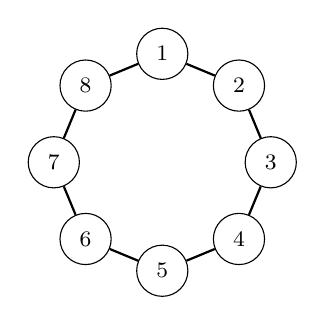
\begin{tikzpicture}[
    scale=0.95,
    every node/.style={
      circle,
      draw=black,
      fill=white,
      inner sep=0pt,
      minimum size=6.5mm,
      font=\footnotesize
    }
  ]
    \def\r{1.45}
    \foreach \i [evaluate=\i as \ang using {90-(\i-1)*45}] in {1,...,8} {
      \node (v\i) at (\ang:\r) {$\i$};
    }
    \foreach \i/\j in {1/2,2/3,3/4,4/5,5/6,6/7,7/8,8/1} {
      \draw[thick] (v\i) -- (v\j);
    }
  \end{tikzpicture}
  \caption{Communication graph.}
  \label{fig:cycle_graph}
\end{figure}

% The communication graph is the undirected graph with the Laplacian matrix
% \begin{equation}
%   L = \begin{bmatrix}
%     2 & -1 & 0 & 0 & 0 & 0 & 0 & -1 \\
%     -1 & 2 & -1 & 0 & 0 & 0 & 0 & 0 \\
%     0 & -1 & 2 & -1 & 0 & 0 & 0 & 0 \\
%     0 & 0 & -1 & 2 & -1 & 0 & 0 & 0 \\
%     0 & 0 & 0 & -1 & 2 & -1 & 0 & 0 \\
%     0 & 0 & 0 & 0 & -1 & 2 & -1 & 0 \\
%     0 & 0 & 0 & 0 & 0 & -1 & 2 & -1 \\
%     -1 & 0 & 0 & 0 & 0 & 0 & -1 & 2
%   \end{bmatrix},
% \end{equation}
% which corresponds a cycle graph.

\begin{figure}[t]
  \centering
  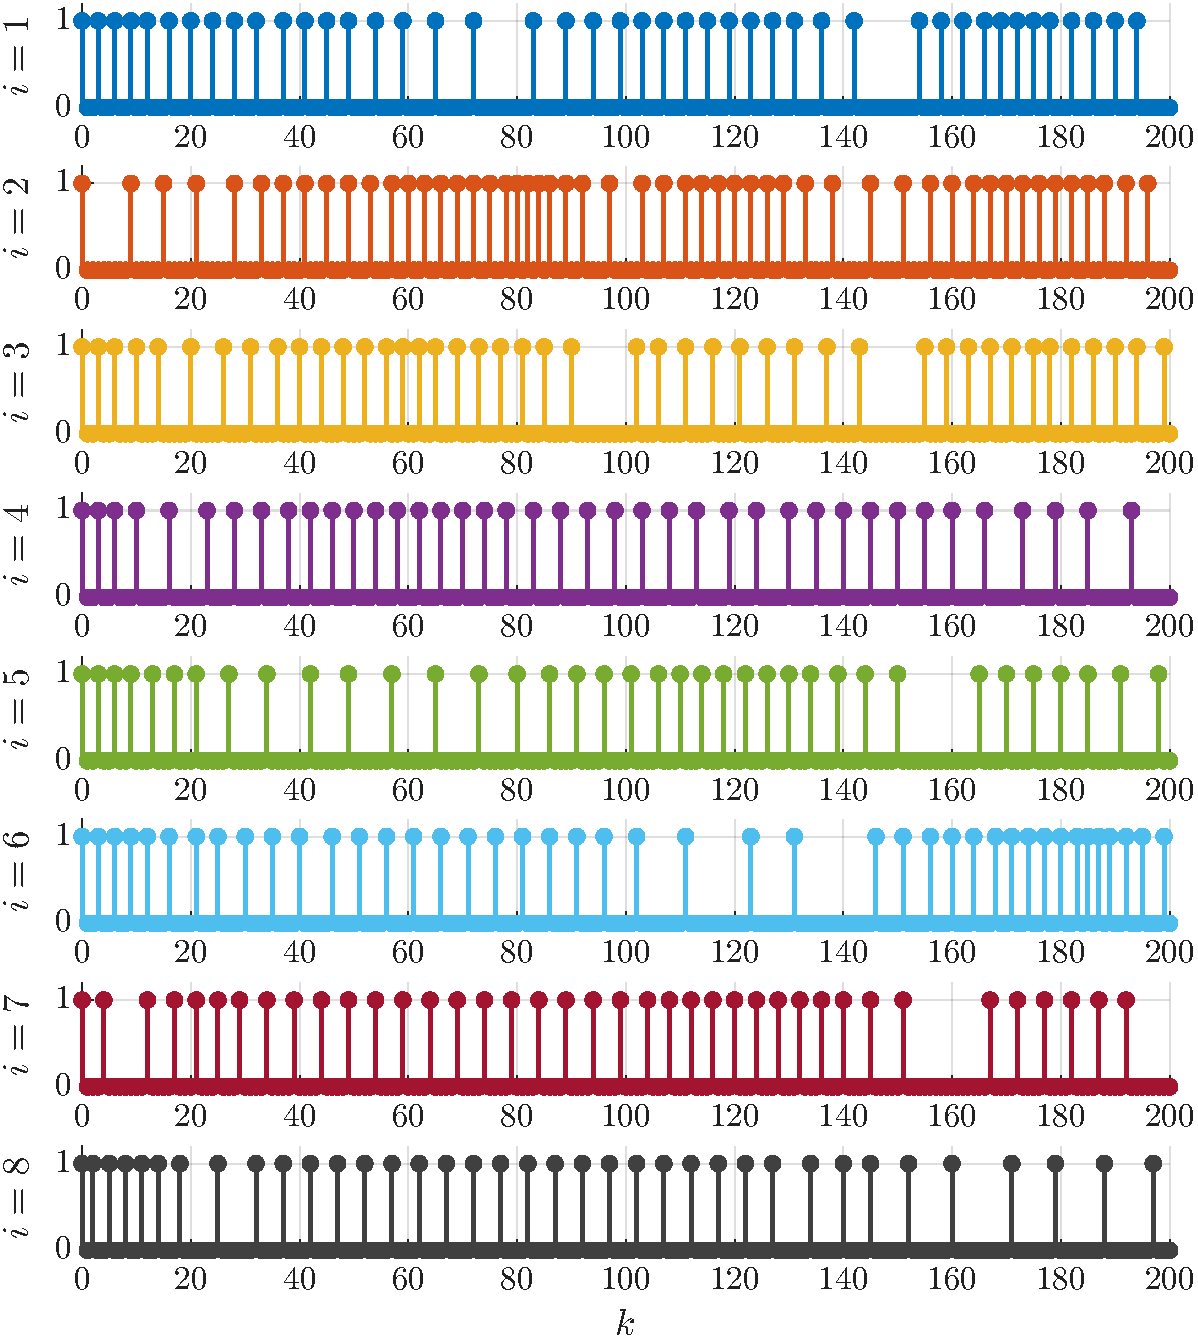
\includegraphics[width=0.98\linewidth]{fig/communication_timings.pdf}
  \caption{Transmission instants of each agent for the proposed event-triggered method, where a value of $1$ indicates that agent $i$ transmits at that time instant, and a value of $0$ otherwise.}
  \label{fig:transmission}
\end{figure}

\begin{figure}[t]
  \centering
  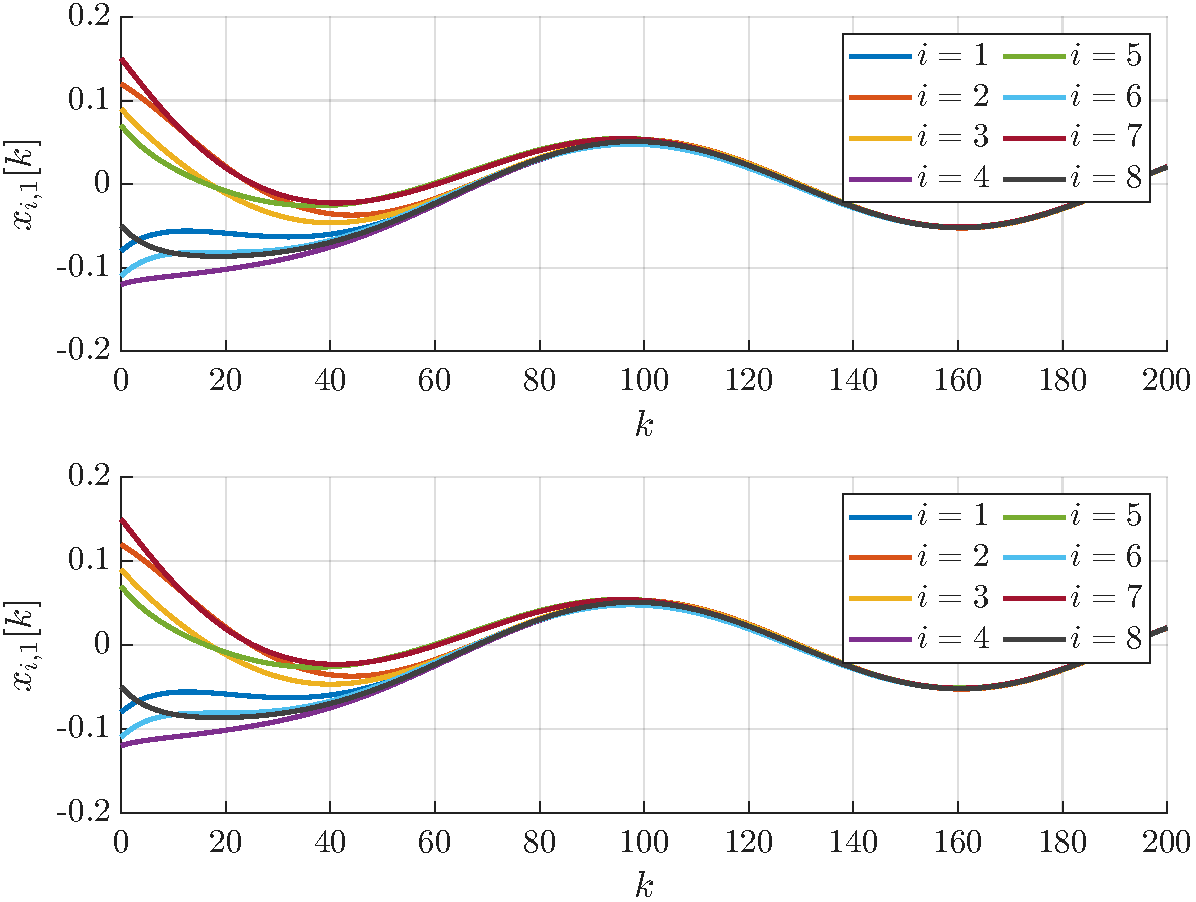
\includegraphics[width=0.98\linewidth]{fig/state_xi-1.pdf}
  \caption{State trajectories $x_{i,1}[k]$ for the all-time communication scheme (top) and the proposed event-triggered method (bottom).}
  \label{fig:state1}
\end{figure}

% \begin{figure}[t]
%   \centering
%   \includegraphics[width=0.98\linewidth]{fig/state_xi-2.pdf}
%   \caption{State trajectories $x_{i,2}[k]$ for the all-time communication scheme (top) and the proposed event-triggered method (bottom).}
%   \label{fig:state2}
% \end{figure}

\begin{figure}[t]
  \centering
  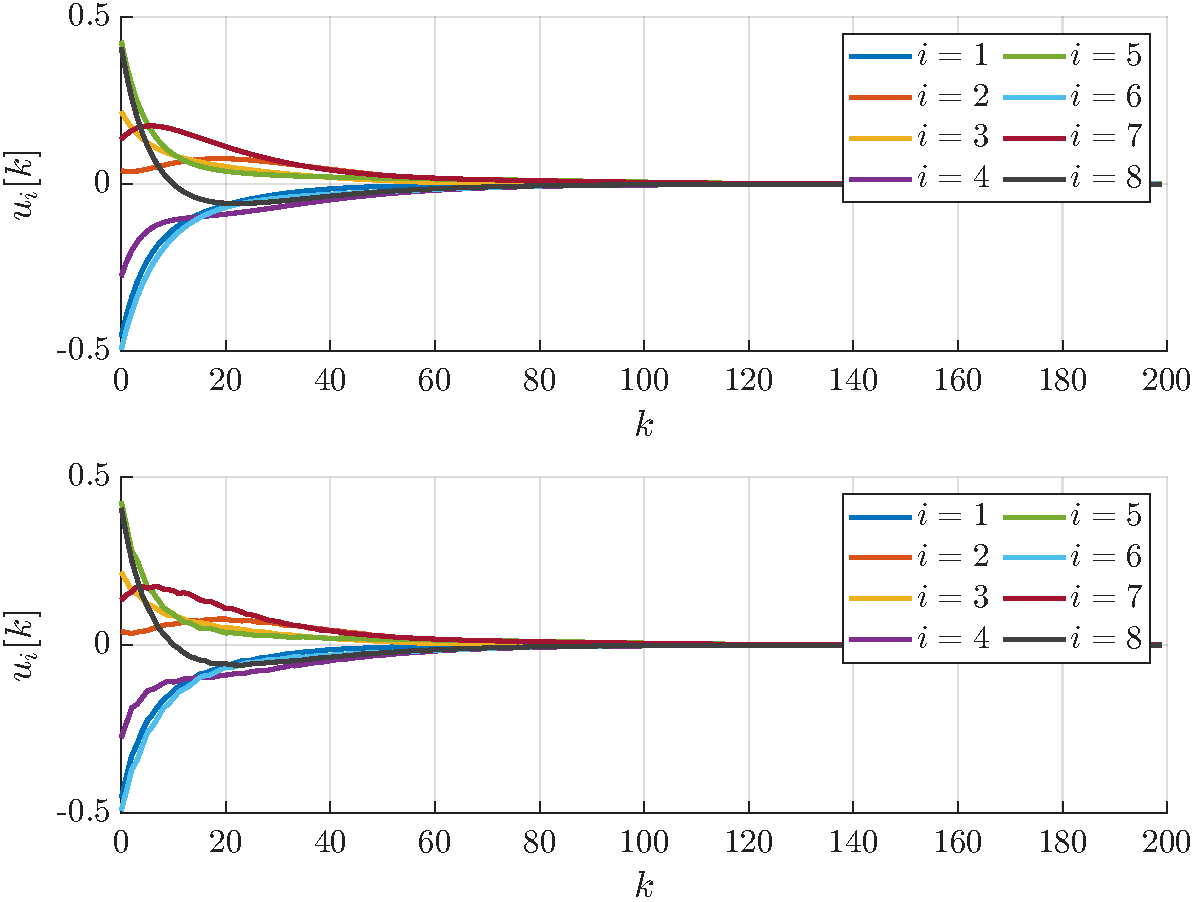
\includegraphics[width=0.98\linewidth]{fig/control_inputs.pdf}
  \caption{Control inputs for the all-time communication scheme (top) and the proposed event-triggered method (bottom).}
  \label{fig:input}
\end{figure}

% \begin{figure}[t]
%   \centering
%   \includegraphics[width=0.98\linewidth]{fig/communication timings.pdf}
%   \caption{Transmission instants of each agent for the proposed event-triggered method, where a value of $1$ indicates that agent $i$ transmits at that time instant, and a value of $0$ otherwise.}
%   \label{fig:transmission}
% \end{figure}

\subsection{Simulation Results}

Fig.~\ref{fig:transmission} illustrates the transmission instants of each agent for the proposed event-triggered method.
As shown in the figure, transmissions occur asynchronously and only at a subset of the time instants.
In the present simulation, transmissions occur at about $20.8\%$ of all possible transmission opportunities across all agents.

Fig.~\ref{fig:state1} depicts the trajectories of the first state component under the all-time communication scheme and the proposed event-triggered method, and Fig.~\ref{fig:input} presents the corresponding control inputs.
These figures show that the proposed method also drives all agents to consensus asymptotically.
In addition, the transient responses under the proposed method remain close to those under the all-time communication scheme over the control horizon.
This indicates that, although the agents communicate intermittently, the resulting closed-loop behavior remains similar to that of the baseline distributed control with all-time communication.

% Fig.~\ref{fig:transmission} illustrates the transmission instants of each agent for the proposed event-triggered method.
% As shown in the figure, transmissions occur asynchronously and only at a subset of the time instants.
% In the present simulation, transmissions occur at about $20.8\%$ of all possible transmission opportunities across all agents.

\subsection{Discussion}

For this numerical example, the proposed method achieves consensus with trajectories close to those of the all-time communication scheme while using only about $20.8\%$ of all possible transmissions.
The realized cost ratio over the horizon $200$ is $J_{\mathrm{etc}}/J_{\mathrm{all}} = 0.9960$, which is well below the prescribed performance level $\rho = 1.2$.
This result suggests the conservatism of the present framework.
The following observations help explain this behavior.

First, Theorem~\ref{th:lq_performance_guarantee} provides only a sufficient condition for $J_{\mathrm{etc}}(x[0]) \leq \rho J_{\mathrm{all}}(x[0])$.
In addition, the global LQ performance constraint must be satisfied through asynchronous triggering decisions based only on locally available information.
Under this information structure, the exact global performance degradation cannot be evaluated directly by each agent, and the analysis in Section~\ref{sec:main_results} relies on scalar worst-case quantities such as $\alpha_S$, $\alpha_{S_u}$, and $\alpha_{\Gamma_U}$.
As a result, the condition is tractable but generally not tight.

Furthermore, the parameter design in Section~\ref{sec:parameter} is heuristic rather than globally optimal.
Accordingly, the obtained parameter $\sigma$ is guaranteed only to satisfy the sufficient condition of Theorem~\ref{th:lq_performance_guarantee}, and is not necessarily the largest feasible value under the given performance constraint.

It is also worth noting that, in this numerical example, the cost ratio satisfies $J_{\mathrm{etc}} < J_{\mathrm{all}}$ even though the proposed method exhibits fewer transmissions than the all-time communication scheme.
As stated in Remark~\ref{rem:local_cost}, $J_{\mathrm{all}}$ is not the globally minimal value of the LQ cost \eqref{eq:lq_cost}.
Moreover, the all-time communication scheme and the proposed method use different information structures to compute their control inputs.
% Hence, the comparison is made between two different distributed controllers under the same performance index \eqref{eq:lq_cost}, rather than between the same controller under different communication rates.
Hence, the proposed method uses more information to compute control inputs than the all-time communication scheme, and a lower communication rate does not necessarily imply a higher LQ cost.

Nevertheless, this numerical example demonstrates the potential of the proposed framework for achieving a favorable trade-off between communication reduction and closed-loop performance.
It also suggests that the conservatism stems from the gap between a global performance requirement and local asynchronous triggering decisions.
Therefore, one possible way to reduce this conservatism is to establish a framework that enables each agent to evaluate the effect of its local triggering decision on the global performance degradation more accurately.

\section{Conclusion}
\label{sec:conclusion}

This paper has studied distributed event-triggered consensus control for discrete-time linear multi-agent systems under an LQ performance constraint.
We proposed a distributed event-triggered control method that guarantees the prescribed level of LQ performance as well as consensus when the triggering parameters are properly designed.
In addition, we presented a tractable parameter design method for obtaining feasible triggering parameters while promoting transmission reduction.
Numerical simulations illustrated that the proposed method achieves consensus with transient responses close to those of the all-time communication scheme while reducing the number of transmissions.
Future work includes reducing conservatism in the theoretical analysis and parameter design, and extending the proposed framework to more general communication settings.

\balance
\bibliographystyle{IEEEtran}
\bibliography{myrefs}

\end{document}
